\documentclass[a4wide,leqno,12pt]{report}
\usepackage[english]{babel}
\usepackage[utf8]{inputenc}
\usepackage[pdftex]{graphicx} %%graphics in pdfLaTeX
\usepackage[export]{adjustbox}
\usepackage{times}
\parindent 0in
\parskip 0.05in
%\usepackage{setspace}
%\doublespacing
\linespread{1.5}
\usepackage{svg}

\begin{document}

\bgroup %% <<<<<<< begin a group
\linespread{0}
\thispagestyle{empty}
\begin{center}
{\sffamily
{\Large University of Dublin}

\vspace{10pt}


\includegraphics[scale=0.12]{images/trinitycollege.pdf}
%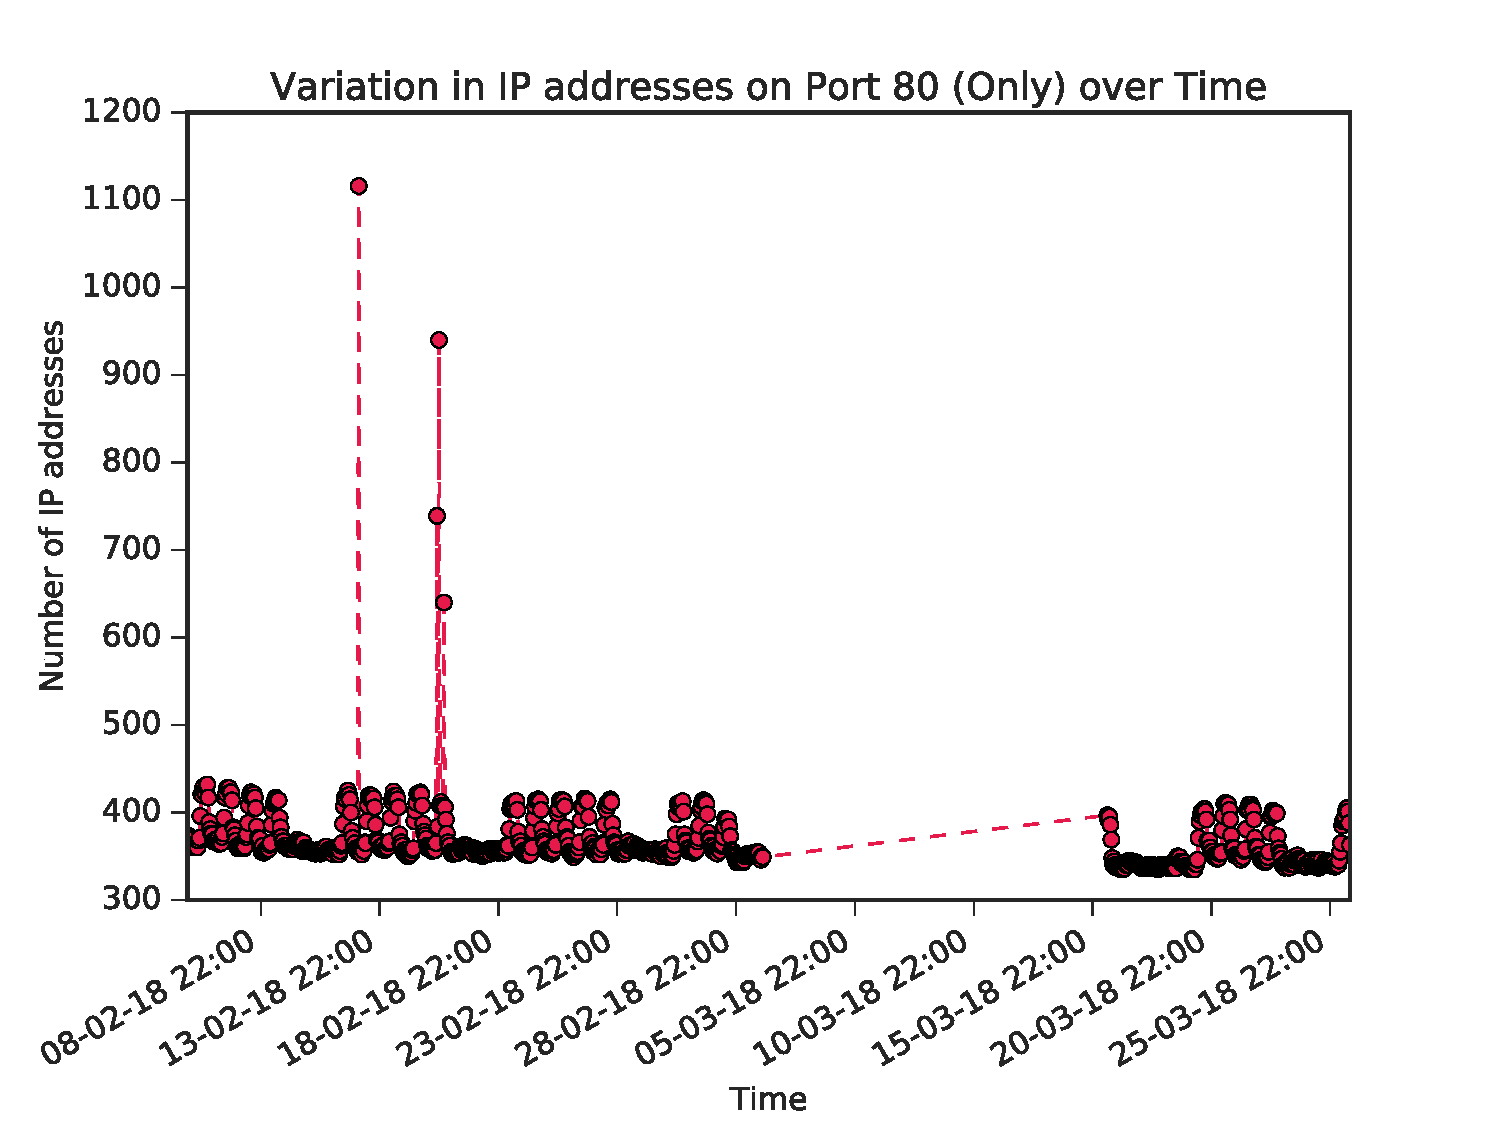
\includegraphics[scale=.5]{t.pdf}

\vspace{10pt}

{\Huge TRINITY COLLEGE}

\vspace{80pt}

\textbf{ \Large \emph A Survey of Web Servers in Trinity College Dublin}

\vspace{30pt}

Michael Power

B.A. (Mod.) Integrated Computer Science

Final Year Project May 2018

Supervisor: Dr. Stephen Farrell

\vspace{110pt}

\large{School of Computer Science and Statistics
\\$ $\\
O'Reilly Institute, Trinity College, Dublin 2, Ireland}
\linespread{1}
}
\end{center}
\egroup %% <<<<<<< end a group

\chapter*{Declaration}
I hereby declare that this thesis is entirely my own work and that it
has not been submitted as an exercise for a degree at any other
university.

\begin{center}
\vspace*{2in}

\underline{\hspace*{3in}} \today

Michael Power
\end{center}

\chapter*{Permission to Lend}

I agree that the Library and other agents of
the College may lend or copy this thesis upon request.

\begin{center}
\vspace*{2in}

\underline{\hspace*{3in}} \today

Michael Power


\end{center}


\chapter*{Acknowledgements}
To be done

\newpage



\pagestyle{headings}
\tableofcontents
\listoffigures


\begin{abstract}
\noindent
As the number of Internet devices grows, so to does the difficultly to monitor these devices effectively. This report details the use of ZMap a port scanner and ZGrab an application banner grabber within Trinity College Dublin To survey Web Servers. System administrators have often hundreds of hosts to consider when monitoring Web Servers. The use of the above tools to audit these Web Servers in order to deal with security issues that if left unattended could potential lead to further problems is of the utmost importance for any organization that aims to mitigate these risks, as well as using these tools to study vulnerabilities in order to better defend from attacks, since the availability of tools such as these leads to the potential of attackers finding vulnerability hosts. Scanning at an Internet wide level has shown great promise for uncovering security problems \cite{durumeric2015search} thus the same should be true at a University Campus level.\\

As well as deploying and testing the tool within Trinity College Dublin, I also hope to be able to interpret the output, and communicate that to site owners/system admins in order to help make their web a bit better and more secure.

\end{abstract}


\chapter{Introduction}
\section{Goals of Report}
!!!!!!!!!!!!!!!MIND TENSE USED (PAST OR FUTURE), PICK ONE AND KEEP IT, ALSO MIND THE USE OF I WHEN DESCRIBING THE REPORT!!!!!!!!!!!!!!!\\



As with any device that is connected to the Internet, the  security of these systems is of concern. Even when following strict policies,  miss configurations of servers can lead to possible issues which could significant impact. The aim of this project is to deploy a local instance of ZMap and ZGrab within Trinity College Dublin, running scans on both port 80 and 443 in order to survey web servers, in an effort to build a picture of what the current state of Web Servers within the college campus looks like.\\

I will also outline the steps that I've taken in order for other organizations and institutions to replicate what I've done here within Trinity College Dublin.\\


This goal will be analyzed with the following questions in mind:
\begin{itemize}
  \item Which IP addresses are listening on port 80, port 443 and both ports?
  \item The variation in the number of host on at a certain time?
  \item How many IP addresses have a Hostname?
  \item What make of servers are being used !!!!!!!!!!!!!!! MORE ABOUT WHO ARE THESE IPS THAT ARE UP, TRYING TO CATEGORISE (WEB IMAGE MONITOR ETC)!!!!!!!!!!!!!!!?
  \item What does the current state of Certificates look like within the college?
  \item Are there any out of date versions of TLS being used?
  \item For those IP addresses that don't have a Hostname, do their certificates lead to one?
  \item What Signature and Key Algorithms are being used?
  \item Is secure renegotiation false for any IP addresses?
  \item Are there any public keys that are used across multiple IP addresses?
  \item The variation in public key lengths?
  \item How many IP addresses are managing redirects correctly?
 
\end{itemize}
\section{Outline}
The remainder of this report is organized as follows:\\
\begin{itemize}
\item\textbf{Chapter 2} provides the reader with the required background information.
\item\textbf{Chapter 3} shows other relevant work conducted in this area.
\item\textbf{Chapter 4} explains the overall design of the investigation as well as the ethical concerns around it.
\item\textbf{Chapter 5} details the implementation of ZMap and ZGrab within Trinity College Dublin as well as describing the various programs and scripts used to gather the data.
\item\textbf{Chapter 6} presents the results of the scans conducted.
\item\textbf{Chapter 7} provides an analysis of the findings in surveying Web Servers within Trinity College Dublin.
\item\textbf{Chapter 8} describes the future work that could be done to extend this project.
\end{itemize}


\chapter{Background}
!!!!!!!!!!!!!!!
\section{Web Server}
!!!!!!!!!!!!!!!REFERENCE RFC FOR HTTP, OR ANY OTHER PORT MENTIONED!!!!!!!!!!!!!!!\\




Web servers are one of components that make up the overall web-application architecture.
Communication between between a web server and a clients browser is done typical through a protocol called Hyper Text Transfer Protocol or HTTP for short. The general way in which a Client initiates communication between a web server is through a Web Browser such as Chrome or Firefox, The browser sends a request to the web sever of some resource typically a web page or some other file type, if the resource doesn't exist an error is returned to the client, generally in the form of a 404 or some other status code. As well as handling request, the server may sometimes be required to handle processing of forms inputted by the client\cite{conallen1999modeling}. Almost any device that is connected to the Internet can host a web server, such as a printer or mobile phone. \\

Web servers play a significant role in terms of the overall workings of web applications and security issues relating to web servers can come in a number of ways such as being incorrectly configured\cite{mendes2008assessing} along with lack of privilege management.
\section{Transport Layer Security}
!!!!!!!!!!!!!!!TALK ABOUT THE THINGS WE ARE LOOKING FOR IN THE TLS, CIPHER SUITE, VERSION ETC!!!!!!!!!!!!!!!\\


TLS or SSL as it may sometimes be referred to is a protocol that allows secure communication between a client and server over the Internet, which is typically between a Browser and Web Server. Over the years there have been many versions of TLS/SSL implementations, the first being in 1994 when Netscape developed SSL 1.O however this was never released publicly as it was vulnerable to replay attack\cite{turner2014transport}. This drove the development of SSL 2.0 in 1995, but along with its predecessor it too had problems. Then in 1996 SSL 3.0 was distributed to combat the issues with SSL 2.0 gaining a large popularity in the process \cite{turner2014transport}. In mid 1996 development of these protocols moved to the Internet Engineering Task Force and so too did the name of the protocol changing from SSL to TLS. To date there have been four releases of TLS with TLSv1 being released in 1999, TLSv1.1 in 2006, TLSv1.2 in 2008\cite{turner2014transport} and in 2014 a draft of TLSv1.3 was developed
 \cite{dierks2014transport}.\\
 \begin{center}
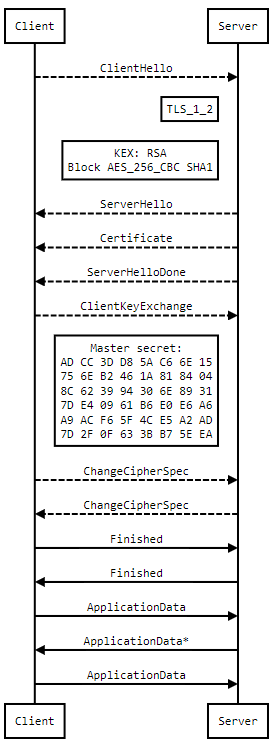
\includegraphics[scale=.5]{images/tls_demo.png}
\end{center}
In order for a secure connection to be established the client first sends a \textit{Client Hello} message which includes the version of TLS supported by the client a random byte string that is used for calculations later on in the handshake such as generating the pre-master secret,  along with the list of cipher suites and compression methods in order of the clients preference \cite{tlsDemoServer}. As well as this the client sends an empty session identifier\cite{turner2014transport}.
The server responds with a \textit{ServerHello} message indicating the version of TLS that will be used along with the appropriate cipher suite, compression method and session Identifier. The server also generates its own random byte string. Next a \textit{Certificate} is sent from the server to the Client whenever the key exchange method uses certificates. This certificate message contains a chain of certificates which the client will use to validate the server says who they say they are. Following this a Server Key Exchange Message is sent if the certificate sent by the server lacks sufficient data for the client to exchange a premaster secret.The Server then sends a \textit{ServerHello Done} message to the Client to signal that the client can now continue with its turn of the key exchange related messages. The Client now sends a \textit{ClientKeyExchange} message to the server which includes the pre-master secret created by the client. Both the Client and the Server send a \textit{ChangeCipherSpec} message to alert each other that all future exchanges within this session will be encrypted with the chosen cipher suite and keys. Finally the Client sends a \textit{Finished} Message to the Server and likewise The Server sends a \textit{Finished } message to the Client, both of theses exchanges are used in order to verify that the key exchange and authentication process were successful as well as indicating that each respective part of the TLS handshake is complete. From this point on all \textit{ApplicationData} exchange between the client and server is protected based on the current connection state \cite{tlsDemoServer}\cite{turner2014transport}
\section{Port Scanning}
!!!!!!!!!!!!!!!!!!!!!!!!!GIVE A MENTION TO OTHER SCANNERS NMAP ETC AS THEHER ARE OTHERS OUT THERE!!!!!!!!!!!!!!!\\
Port scanners are tools that are used to check for devices on open ports, these tools could be used by system administrator to monitor devices on a network or by a malicious party hoping to find vulnerable devices to infect. \\
There are three main grades of port scans.
\begin{enumerate}
\item\textbf{Vertical Scans:}
The vertical port scan is one in which a single host is scanned across mulitple ports.
\item\textbf{Horizontal Scans:}
The horizontal scan is one in which a single port is scanned against multiple hosts.
\item\textbf{Block Scans:}
The Block scan is a combination of vertical and horizontal scans.\cite{lee2003detection}
\end{enumerate}
\subsection{ZMap}
!!!!!!!!!!!!!!!REFERENCE UDP, BACKNET ANYTHING THAT IS NOT OBVIOUS FOR FURTHER CLARIFICATION OR ANYTHING THAT IS GOING TO BE TALKED ABOUT IN THE RESULTS!!!!!!!!!!!!!\\


!!!!!!!!!!!!!! SHOW AND DESCRIBE SAMEPLE OUTPUT !!!!!!!!!!!!!\\




ZMap is an open-source network scanner optimized for efficiently performing
Internet-scale network surveys \cite{durumeric2013zmap}, developed in 2013 by Zakir Durumeric, Eric Wustrow and J. Alex Halderman at the University of Michigan they have been able to effectively diminish the time required to scan the IPv4 address space to a matter of minutes. The architecture allows sending and receiving components
to run asynchronously and enables a single source machine to comprehensively scan every host in the public IPv4
address space for a particular open TCP port in under 45 mins using a 1 Gbps Ethernet link\cite{durumeric2013zmap}. The default configuration for ZMap unfortunately only allows scans for one specified port in the given IP range (CIDR Block), which in our case and many others requires users of this tool to write further programmes to investigate hosts on more than one specified port. ZMap currently has fully implemented probe modules for TCP SYN scans, ICMP, DNS queries, UPnP, BACNET, and can send a large number of UDP probes \cite{zmapGithub}\\


In order to randomise the scans conducted on the target address space, ZMap remains stateless. To avoid keeping state ZMap sends a fixed number of probs per target with the default sending only one probe.\cite{durumeric2013zmap}\\

One of the problems of Internet wide scanning is that it uses a large amount of bandwidth,
the creators of ZMap have introduced seven points in relation to the best practices when conducting these scans\cite{durumeric2013zmap} page 12. \\


\begin{center}
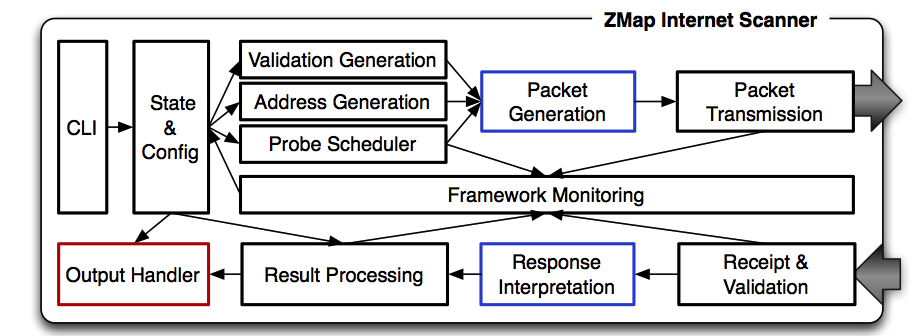
\includegraphics[scale=.4]{images/zmap_architecture.png}
\end{center}

Figure 1. ZMap Architecture.\\


ZMap uses a modular design to support many types of probes and integration with a variety of research applications. Instructions are entered Via the Command Line (CLI) which are then parsed to the \textit{State \& Config} module. The next two modules \textit{Validation Generation} and
\textit{Address Generation} are responsible for generating the target space/address range while also validating this space to ensure any host/IP addresses are excluded according to a configuration file which omits sites/IP ranges such as any reserved address allocations along with others who may wish to opt out of future scans \cite{durumeric2013zmap} while the \textit{Probe Scheduler} sets the timing of the soon to be sent probes. Next we have the \textit{Packet Generation} module which is responsible for generating the required probe packets as per the type of scan we are conducting , the \textit{Packet Transmission} module is responsible for sending these packets to their intended destination. ZMap also provides Extensible probe modules which can be customized for different kinds of probes, and are responsible for generating probe packets and interpreting whether incoming packets are valid responses. The \textit{Framework Monitoring} oversees every packet that is sent and received, while the \textit{Receipt \& Validation} module responds to TCP SYN-ACK packets and discard packets clearly not initiated by the scan by cross checking the source and destination ports of the packets. The \textit{Response Interpretation”} interprets the responses from those that have been validated by the \textit{Receipt \& Validation} module. Before the results of the probes are outputted they are first brought to the \textit{Result Processing} module which processes the results and outputs these either to the console via stdout or to be piped to another process directly such as ZGrab or outputted to a comma separated file (csv) \cite{durumeric2013zmap}.\\

The speed at which ZMap sends packets is performed as fast as the source's CPU or NIC allows. This speed however at which ZMap sends probes is a cause for concern, as sending them in numerical order would probably overload and cause a network failure. So in order to counteract this ZMap uses a random permutation of the address space, iterating over a multiplicative group of integers modulo p, with p being slightly larger than $2^{32}$. By choosing p to be a prime, ZMap guarantees that the group is cyclic and
will reach all addresses in the IPv4 address space once per cycle. To select a new permutation for each scan, a new primitive root of the multiplicative group and a new random starting address are chosen. ZMap efficiently finds random primitive roots of
the  multiplicative  group  by  utilizing  the  isomorphism $(Zp - 1,+)~=(Z*p,x)$ and  mapping  roots of$(Zp-1,+)$ into the multiplicative group via the  function f(x) =nx where n is a known primitive root of$(Z/pZ)x$. Once this primitive root is ZMap cycles through the target address space by applying the group operation to the current address. The scan is finished once the initially scanned IP address is reached\cite{durumeric2013zmap}.\\

ZMap send packets at Ethernet Level in order to cache packet values and reduce to overhead on the Kernel.
ZMap implements a probing technique known as
SYN scanning or half-open scanning \cite{durumeric2013zmap}. This was chosen to instead of performing a full TCP handshake
based on the reduced number of exchanged packets.  In
the situation where a host is unreachable or does
not respond, only a single packet is used in the exchange (a SYN from
the scanner); in the case of a closed port, two packets
are exchanged (a SYN answered with a RST); and in the
situation where the port is open, three packets are
exchanged (a SYN, a SYN-ACK reply, and a RST from
the scanner which will close the connection)\cite{durumeric2013zmap}.


\section{Banner Grabbing}
Banner grabbing is a technique used to gain information about a device on a network by establishing a connection and observing the output from the connection \cite{kondo2014penetration}. System Administrators can use these tools designed for this application to take inventory of the devices and services on their network. Attackers can also use banner grabbing tools in order to find network devices that are using known applications with well documented vulnerability (MD5 for example)


\subsection{ZGrab}
!!!!!!!!!!!!!! SHOW AND DESCRIBE SAMEPLE OUTPUT !!!!!!!!!!!!!\\

ZGrab is one such banner grabber implemented in go that allows user to perform various application handshakes for a number of different protocols such as HTTP, HTTPS, SSH as well as SMTP to name a few. ZGrab connects to the host by opening up a TCP connection. ZGab outputs the information in raw JSON format retrieving all the information about the connection handshake such as SSL/TLS information as well as response codes.\cite{durumeric2015search}

For example When performing a TLS handshake with a host, ZGrab offers the cipher suites implemented by the Golang TLS library and logs the chosen cipher suite\cite{durumeric2015search} rather than using the chosen cipher suite of the source machine performing the ZGrab . ZGrab can be also be used inconjuction with ZMap to grab information simultaneous while a host being scanned or independently of ZMap by passing the host directly into ZGrab. Instructions are passed to ZGrab much in the same way of ZMap via a command line interface (CLI)


\chapter{Related Work}
Other similar scanning works can be seen with Zakir Durumeric, Michael Bailey and J. Alex Halderman the creators of ZMap/ZGrab at the University of Michigan,  where in 2014 \cite{durumeric2014internet}, they published a paper relating to the overall environment of scanners on the Internet by analysing a years worth of data from January 1st 2013 up until May 1st 2014 from a large network telescope revolving around scanning activity with a scan being defined as an "instance where a source contacted at least 100 unique addresses in our darknet(.0018\% of the public IPv4 address space) on the same port and protocol at the minimum estimated Internet-wide scan rate of 10 packets per second (pps)", they also investigated the way in which organisations were protected themselves against these scans if at all. Motivations behind the many of scans that they discovered were in relation to academic research, while a large proportion of scans were targetting services with know vulnerabilities (e.g. SQL serves). Throughout this period 10.8 million scans from 1.76 million hosts were detected with the distribution of the scans found being 56.4\% TCP SYN packets, 35.0\% UDP packets, and 8.6\% ICMP echo request packets. The HTTP and HTTPS are among the highest in terms of number of scans found on these protocols which in relation to my own project are the protocols most familiar with port 80 and 443. With malicious users and attackers having the ability to use these tools for various rouge purposes scan detection plays a huge part in defending organisations however according to this paper the vast majority don't regard scanning as a significant threat, that being said within 24 hours of new vulnerabilities being released on devices, they discovered an increase in the number of scans conducted on the ports commonly associated with those devices for example regarding the disclosure of the Heart-bleed Bug which was discovered in March 2014 and publicly disclosed on April 7th 2014. The vulnerability itself allows attackers to remotely dump arbitrary private data from many common and popular servers that support TLS. In the week following the public disclosure 53 scans from 27 host targeting HTTPS were observed, prior to the disclosure of the vulnerability 29 scans from 16 hosts were observed targeting HTTPS.\\

The University of Michigan performs regular scans for HTTPS hosts\cite{durumeric2014internet} in order to track the certificate authority ecosystems in an effort to analyse TLS certificates and the Certificate Authorities that sign them. Between the periods of April 2012 and June 2013 they managed to collect 33.6 million unique X.509 Certificates of which 6.2 million were browser trusted as well as identifying the most common CAs by leaf certificates issued, with GoDaddy.com, Inc accounting for 31\% adoption rate of the HTTPS protocol throughout their scans with an increase of 23\% in the Alexa Top 1 million websites and  10.9\% increase in the number of browser-trusted certificates. Keys and Signatures were also tracked to highlight how ZMap could also be used to mitigate risk and act as defensive tool for researchers but this also has the flip side effect of an attacker using this tool to locate hosts suffering from a new vulnerability within minutes.\cite{durumeric2013zmap}  With the research still finding some Certificate Authorities still using MD5 to sign their certificates \cite{durumeric2013analysis}. Within the scope of my own project, I will also be investigating the certificates found within the University, looking at certain parameters such as the signature algorithm used to sign the certificate along with the number of self signed and browser trusted certificates within the University.  \\


Censys begun in 2015 and is a platform created by the same team that designed ZMap that helps information security practitioners answer security related questions in an effort to discover new threats and assess there impact they may have. They regularly probe every public IP address and popular domain names through horizontal scans of the IPv4 address space, curating data over time to see changes in protocol adaption for example, and make it accessible through an interactive search engine and API that allows users to ask questions such as "what percentage of HTTPS servers support SSLv3" by eliminating the labour intensive process of analysing gigabytes of data as well as lowering the barrier to entry for researchers who might not have the performance capabilities to perform these scans.\cite{durumeric2015search} they have also played a central role in the discovery or analysis of some of the most significant Internet-scale vulnerabilities: FREAK, Logjam, DROWN, Heart bleed, and the Mirai botnet. Today however Censys has moved out of the University of Michigan and into it's own company in order to better serve and expand their capabilities to research offering more enhanced services, technical support, and an even more complete and powerful view of the Internet \cite{censysWeb}.
Censys could also be used to identify public facing devices that may have been intended to be private within a network but unintentional found it's way to public INTERNET or be used to calculate the risk that known public facing device could have on an organisation \cite{durumeric2015search} by using their website to investigate such questions.\\


In conjunction with researchers at the University of Michigan, researchers at The International Computer Science Institute and the University of Illinois Urban-Champaign in 2016 have conducted similar HTTPS surveys but by analysing certificates from a large body of sources instead of just one with an aim to obtain a better perspective of the HTTPS ecosystem. In total they combined 8 different data sets observing nearly 17 million unique browser trusted certificates which were valid during August 29 to September 8, 2016 which was the investigation period of their study. Of the 8 datasets analysed Censys(38\%) and CT logs(90.5\%) accounted for 99.4\% coverage of all certificates observed. They are currently working with both parties in order to reduce the discrepancy between either source in order to make each one more or less a near comprehensive view of trusted HTTPS certificates\cite{vandersloot2016towards}.\\

Researchers at Ajou University, have  implemented ZMap within their own University campus in aid of identifying hosts and comparing various scanning techniques such as FIN and Xmas Scans for identifying hosts by conducting scans on a number of ports including port 25 (smtp) , 80(http) and 443 (https). These optional scanning techniques are implemented by creating specific probe modules for ZMap \cite{lee2016implementation}. Some of the hosts they discovered included old web servers of a printers which allowed them to instruct the printer to print test pages as well as gaining access to  password protected content of the printer with default passwords of the known devices still in use and common on the Internet. While this Report on the other hand uses exclusive SYN scanning the default for ZMap with an aim to identifying regular and irregular Hosts running on port 80 and 443 as well analysing the current configurations of these Web Servers within the university, I was hope to discover similar devices on these ports that were found in Ajou University among others.\\

This report differs from previous studies in terms of the scope of our dataset as well as the direct line of the questions we intend to answer in order to highlight the state of Web Servers within TCD.

\chapter{Design}

\section{Overview}
\begin{figure}[h!]
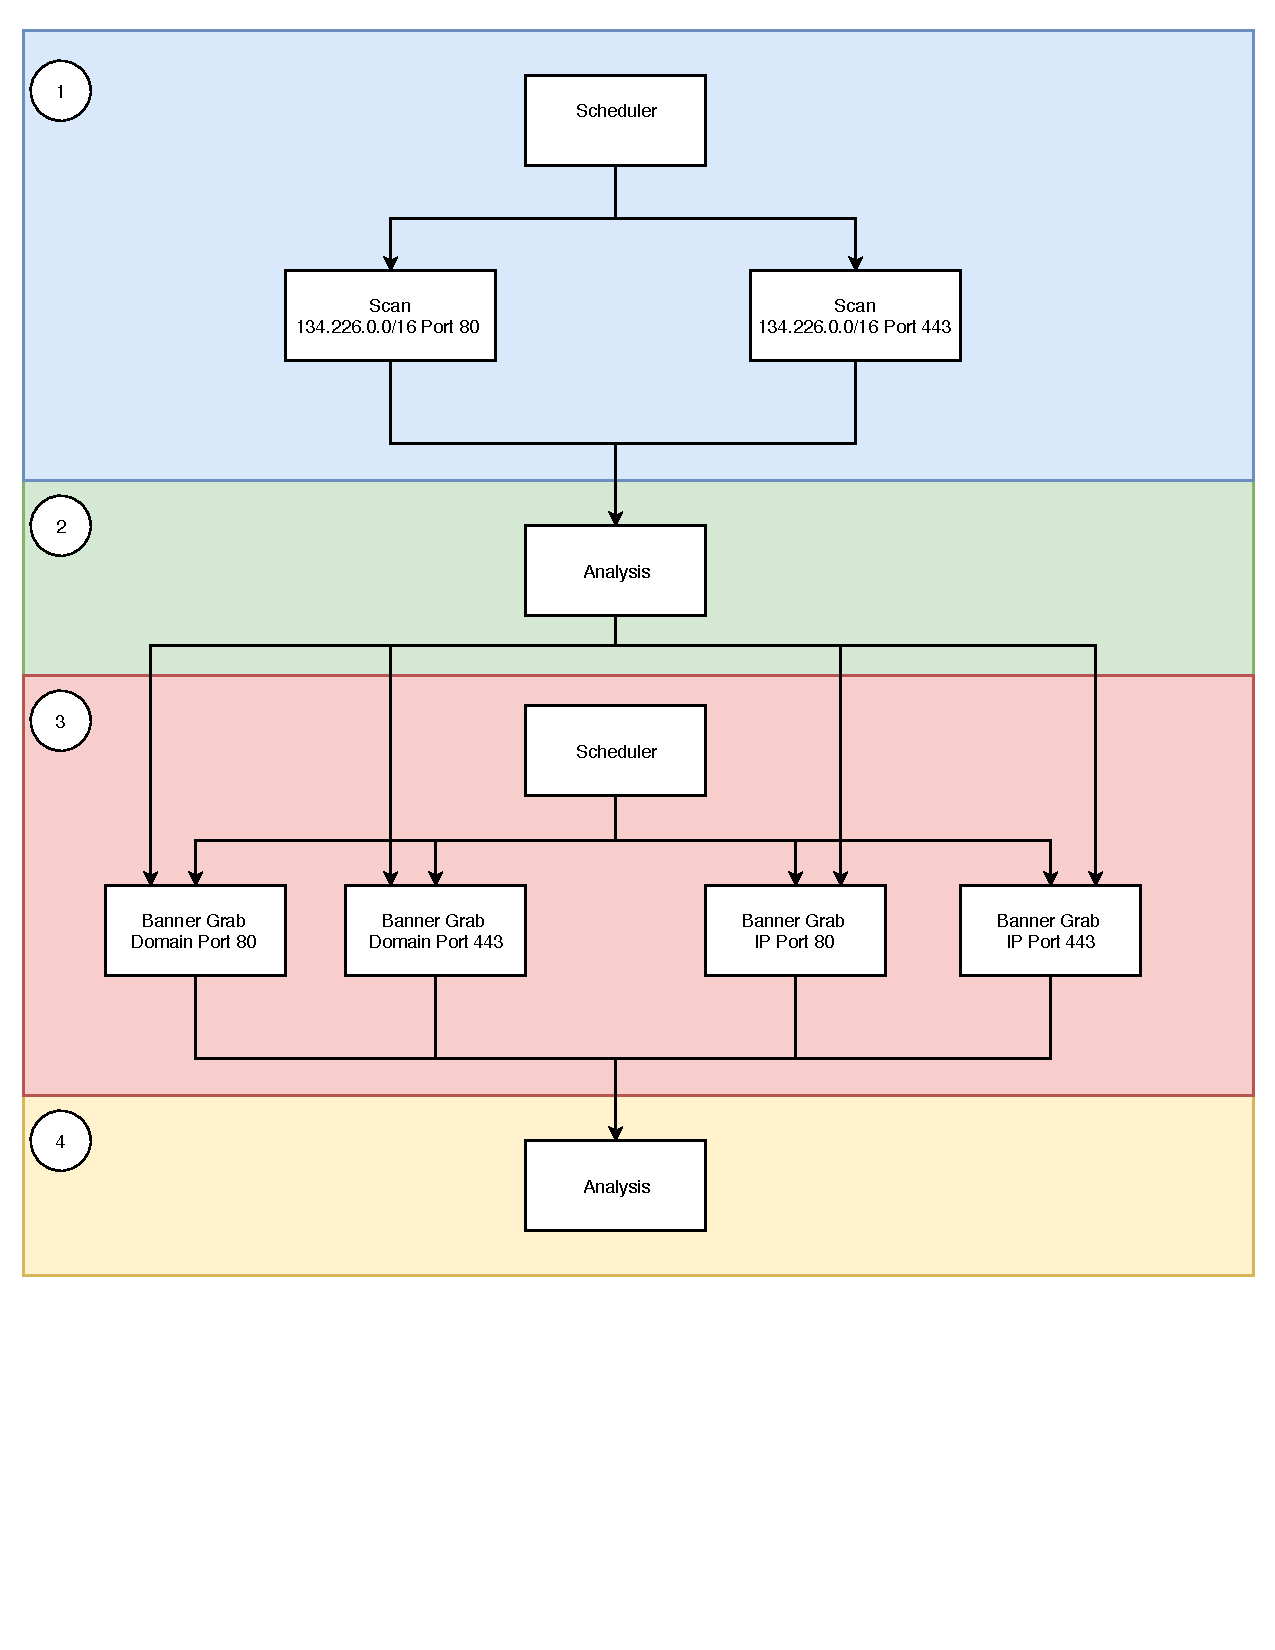
\includegraphics[scale=.5]{pdf_images/design}
\caption{a nice plot}
\label{fig:design}
\end{figure}

As we can see from figure \ref{fig:design} in section 1 highlighted in blue,
the design of the scans consisted of two horizontal set of scans on port 80 and port 443 that would run every hour being executed by a scheduler. After this we would analyse the raw data outputted by ZMap in section 2 in green, once we discovered which IP addresses were listening on which Port along with which IP had an associated host name by doing a reverse DNS lookup in order for us to conduct the ZGrab scans with a domain lookup. Once the data was sufficiently analysed, we conducted 4 sets of ZGrab scans, which were a domain lookup on port 80, a domain lookup on port 443, IP banner grab on port 80 as well as port 443, seen in section 3 of figure \ref{fig:design}. Lastly the output of the ZGrab scans would be analysed looking for certain fields that would be of interest.

\section{Ethics}


As with any type of scanning work that is being conducted, there are a number of ethical considerations to be aware included how the scans should be conducted. We informed the system administrators within the college, stating the intent of the scans that we were conducting. We also decided to limit the port that would be scanned to port 80 and port 443 to limit the strain that the scans could potentionally have on the network. While there are no codes of conduct as of yet in relation to scanning network, the creators of ZMap offer a few useful best practice guidelines when performing scans\cite{durumeric2015search}  \cite{durumeric2013zmap}.\\

Another consideration to account for is the releasing of data, since the majority of hosts are not publicly visible, for this reason no individual IP addresses are released in the report.
\chapter{Implementation}

!!!!!!!!!!!!!!!put in Github link in this section!!!!!!!!!!!!!!!\\

This chapter will cover the implementation of the scans and banner grabs conducted in this project
\section{Technologies Used}
The majority of this project was implemented in Python and Shell scripts, here I list the main technologies used:
\begin{itemize}
  \item ZMap as discussed earlier is a port scanner that finds IP addresses listening on a port by searching an IP/IP range against the desired port.
  \item ZGrab is used to perform the banner grabs of the IP addresses found.
  \item Crontab was used to automate/schedule both the ZMap and ZGrab.
  \item The majority of Python code was used to analyse and sort the data , as well leverage some libraries with python such as the socket library \cite{socket} to perform both DNS and reverse DNS lookup.
  \item Shell Scripts programmes were used to package ZMap and ZGrab in order for it to run with crontab.
  \item Matplotlib \cite{matplotlib} is a python library used to plot the graphs in this report.
\end{itemize}

\section{ZMap Implementation}
In order to implement the ZMap scans as discussed in the design in Chapter 4, I packaged ZMap within a Shell Script that would be set to run every hour on the hour by crontab which is a time based Scheduler in linux. The ouput of the two ZMap scans would be appended to a csv file lying in the server.\\

To differentiate which IP addresses were listening on to one or more ports I created a python programme to find what IP addresses were listening on Port 80 and which IP addresses were listening on Port 443 doing this I was able to get the intersection of the Two to determine the number that were listening on both Ports. The way in which I found out which IP addresses were actually listening to only port 80, port 443 and which were listening to both ports I used a key value dictionary to determine this with the key being the IP address and value being a list of Ports that particular IP address was one for example an IP address that was listening to only port 80 would have a value of [‘80’] likewise for an IP address that was only listening to port 443 would have a value of [‘443’] and for an IP address that was on Both ports would have a value of [‘80’,’443’] .

In order to determine what IP address resolved to hostname in order to do a ZGrab with a domain to determine if there where any different Certificate Alt names between the IP lookup and its corresponding Domain Name. To implement this I used the socket library within python to do a reverse DNS lookup to obtain the hostnames.\\


\section{ZGrab Implementation}

To Implement the ZGrab scans took a bit more care as different types of machines would have different fields present in some and not in others, this was discovered by testing a few machines which we controlled on both sides in order to get a collection that would be of interest to us. These machines were as follows:

\begin{itemize}
  \item A site that was signed by A Certificate Authority.
  \item One that was self Signed.
  \item A 2006 printer on Port 80.
  \item A site that wasn't being maintained.
  \item As well as a two IP addresses on Port 80 and 443.
 
\end{itemize}


!!!!!!!!!!!!!!!PLACE ERROR FILE OF ZGRAB JSON OUTPUT AS AN EXAMPLE!!!!!!!!!!!!!!!\\

These banner grabs that were conducted helped us in order to see the difference of the JSON outputs that ZGrab gives. Similarly for the ZGrabs I've implement much in the same for the ZMap scans, instead here we are also doing the domain lookups as well on port 80 and port 443. To extract the fields I was interested in I implemented a pyhton programme that would take the JSON output of the ZGrab and collect those fields we wanted. In order to take account for the fields that could be present in any practicular ZGrab output, exception handling was conducted on fields were attempting to extract the fields, this was also necessary due to the fact that if certain IP wasn't on at the time a ZGrab was being conducted an error would be outputted in the JSON file along with the IP of the ZGrab that was just executed, with the fields we were concerned with being absent.
\section{Challenges}
One of the Challenges that was encountered is the scheduling of the cron jobs for ZGrab. Throughout ZGrab's conducted not all of the original IP addresses that were found in the ZMap scan presented themselves in the ZGrab data this can be contributed to a number of different reasons, One of these is the fact that the college has a number of IP address that are up less than 90\% of the time period for which ZMap scans were conducted as well as ZMap being run every hour on the hour, where as in the original scheduling of ZGrab they were set up to run for every 2 hours on the hour and as a result the hours on either side might have have presented themselves with IP address that are only in those slots. The reason this was done to run every 2 hours was due to ZGrab taking some time to complete a banner grab especially when an IP or domain wasn't up causing ZGrab to wait for a default of 10 seconds before attempting to abandon the connection. Releasing this I decided to reduce the default timeout to 5 seconds as  well as running multiple ZGrabs over smaller list of IPs or domains every hour rather than a single ZGrab being conducted for instance on the either list of IP addresses on port 443 but rather splitting that list of IP addresses on port 443 into 2/3 smaller list with a dedicated ZGrab Script being executed by the crontab. These methods improved the proformance of the ZGrab allowing us to implement more frequent ZGrabs on smaller lists.

\chapter{Results}

For Comparison of Some results e.g average host per hour look at page 5 and 6 of \cite{durumeric2013zmap}\\

Other comparison \cite{durumeric2015search} page 9 percentage of cipher suites being used could have a new column with TCD figure 5\\

Another comparison can be found with \cite{lee2016implementation} on page 683 finding out of date printers that haven't been updated in a long time\\

Another comparison can be found with trying to see how many scans are necessary for discovering all the host \cite{durumeric2013analysis} page 4\\

Another result comparison could be trying to identify CA that sign certs who have had security issues in the past \cite{durumeric2013analysis} page 6\\

Another result comparison could be looking at key lengths \cite{durumeric2013analysis} page 7 and 8, also look for a paper with recommendations of cryptographic algorithms and key lengths\\

Another result comparison could be looking at signature algorithms, algorithms used to sign the certificates \cite{durumeric2013analysis} page 9\\

Another result comparison looking at ips/hosts sharing multiple public keys, certs e.g Stephens Research and \cite{durumeric2013analysis} page 10\\

Another result comparison could be seeing sites vulnerable to FREAK Attack \cite{vandersloot2016toward} page 54
vandersloot2016toward7\\


In this section we will
present the results of the scans and use them to answer the questions outlined in section 1, in order to better understand the state of Web Servers in the college.


\section{ZMap Results}
!!!!!!!!!!!!!!!!!FIND PERIODS WHEN SERVER WAS DOWN !!!!!!!!!!!!!!!!!!!!!!!!!

\begin{figure}[h!]
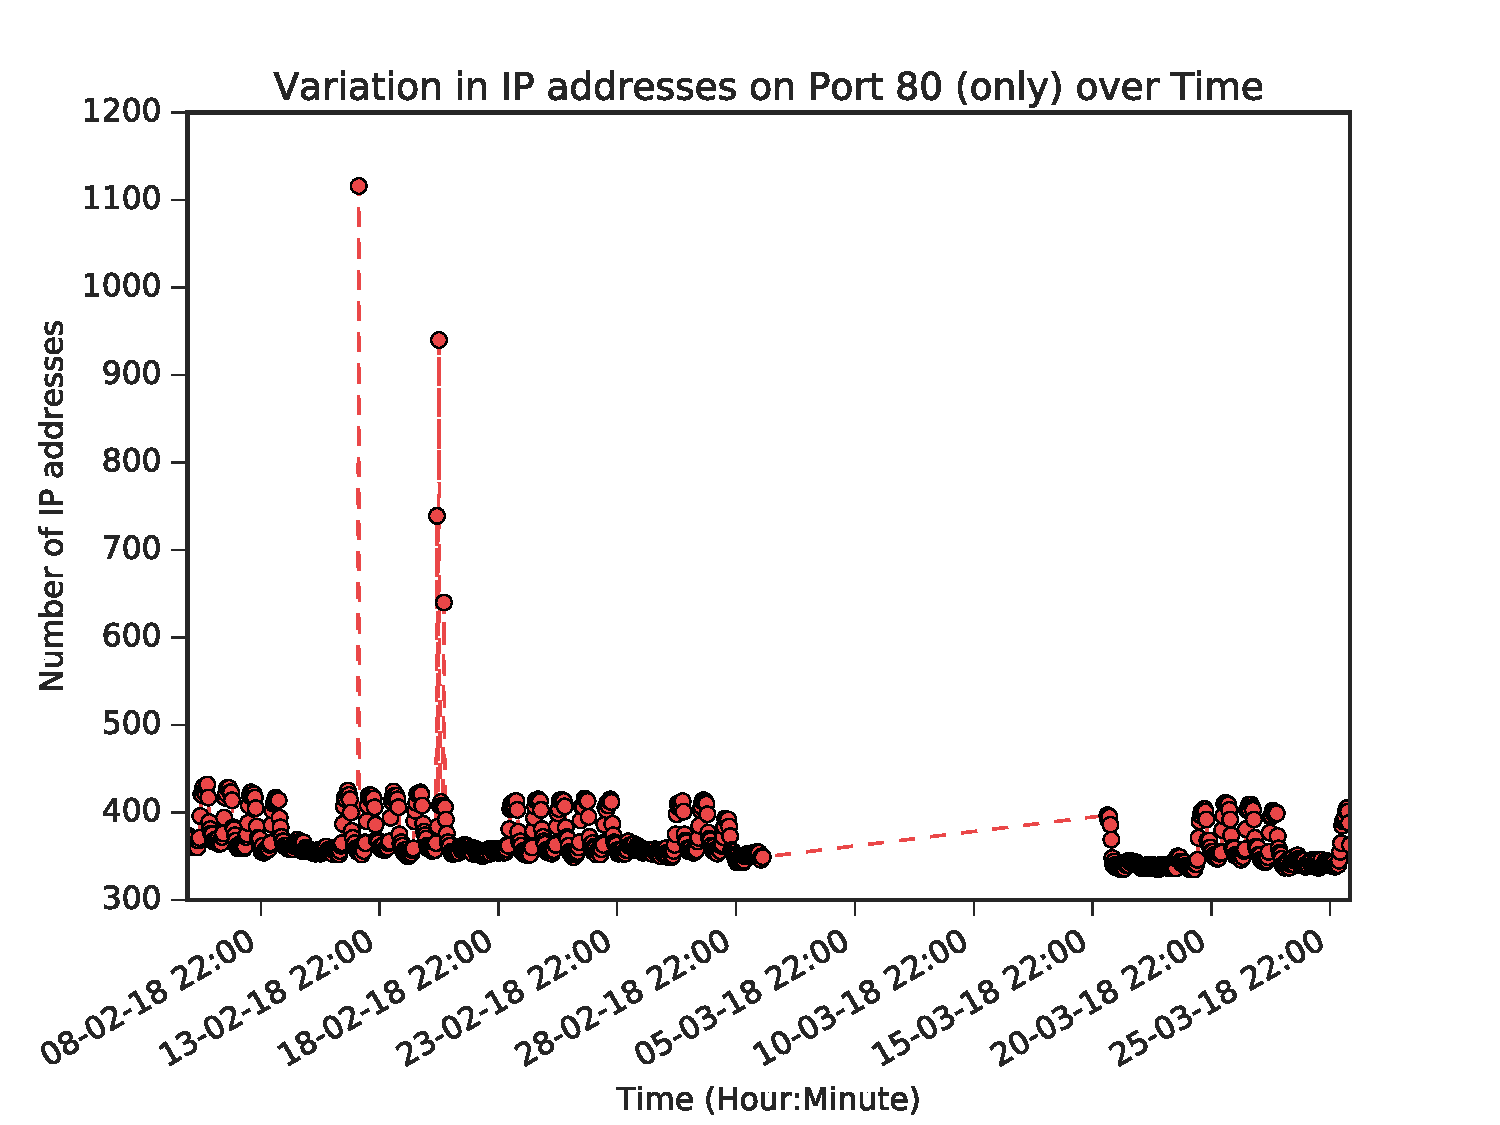
\includegraphics[scale=.5]{pdf_images/VariationInIpAddressesOnPort80OverTime}
\caption{a nice plot}
\label{fig:port80ZMap}
\end{figure}

The ZMap scans took place between the 5th of February at 8pm up until and including the 26th of March at 6pm. However as we can see in figure \ref{fig:port80ZMap} during the periods
02-03-2018  up until 16-03-2018 no scans were detected as this was during the snow period which caused a power cut in the college, downing  Stephen's Server that was conducting the ZMap Scans on both Port 80 and 443. In absence of this there was a total of 827 observational periods in which the ZMap scans took place. We can also see in figure \ref{fig:port80ZMap} an exceptional high count of 1116 IP addresses was recorded on the 13th of February at 1am (2018-02-13T01), this high count was due to an unknown failure of the ZMap scan on port 443, as within this observational slice there were no subsequent IP addresses on port 443 to compare against.
\begin{table}
\centering
\begin{tabular}{||c c c c ||}
 \hline
  & Port 80 (only) & Port 443 (only) & Both Ports \\ [0.5ex]
 \hline\hline
 Monday & 367 & 383 & 377  \\
 Tuesday & 378 & 383 & 377 \\
 Wednesday & 377 & 383 & 377 \\
 Thursday & 372 & 383 & 377  \\
 Friday & 383 & 383 & 377 \\
 Saturday & 352 & 383 & 377\\
 Sunday & 349 & 383 & 377\\[1ex]
 \hline
\end{tabular}
\caption{Average Number of IP addresses across week}
\label{table:1}
\end{table}

Another intriguing  point to note is that the count of IP addresses throughout the week is steady, with the number of IP addresses on port 80 (only) rising throughout the weekdays and falling at the weekend.\\

\begin{figure}[h!]
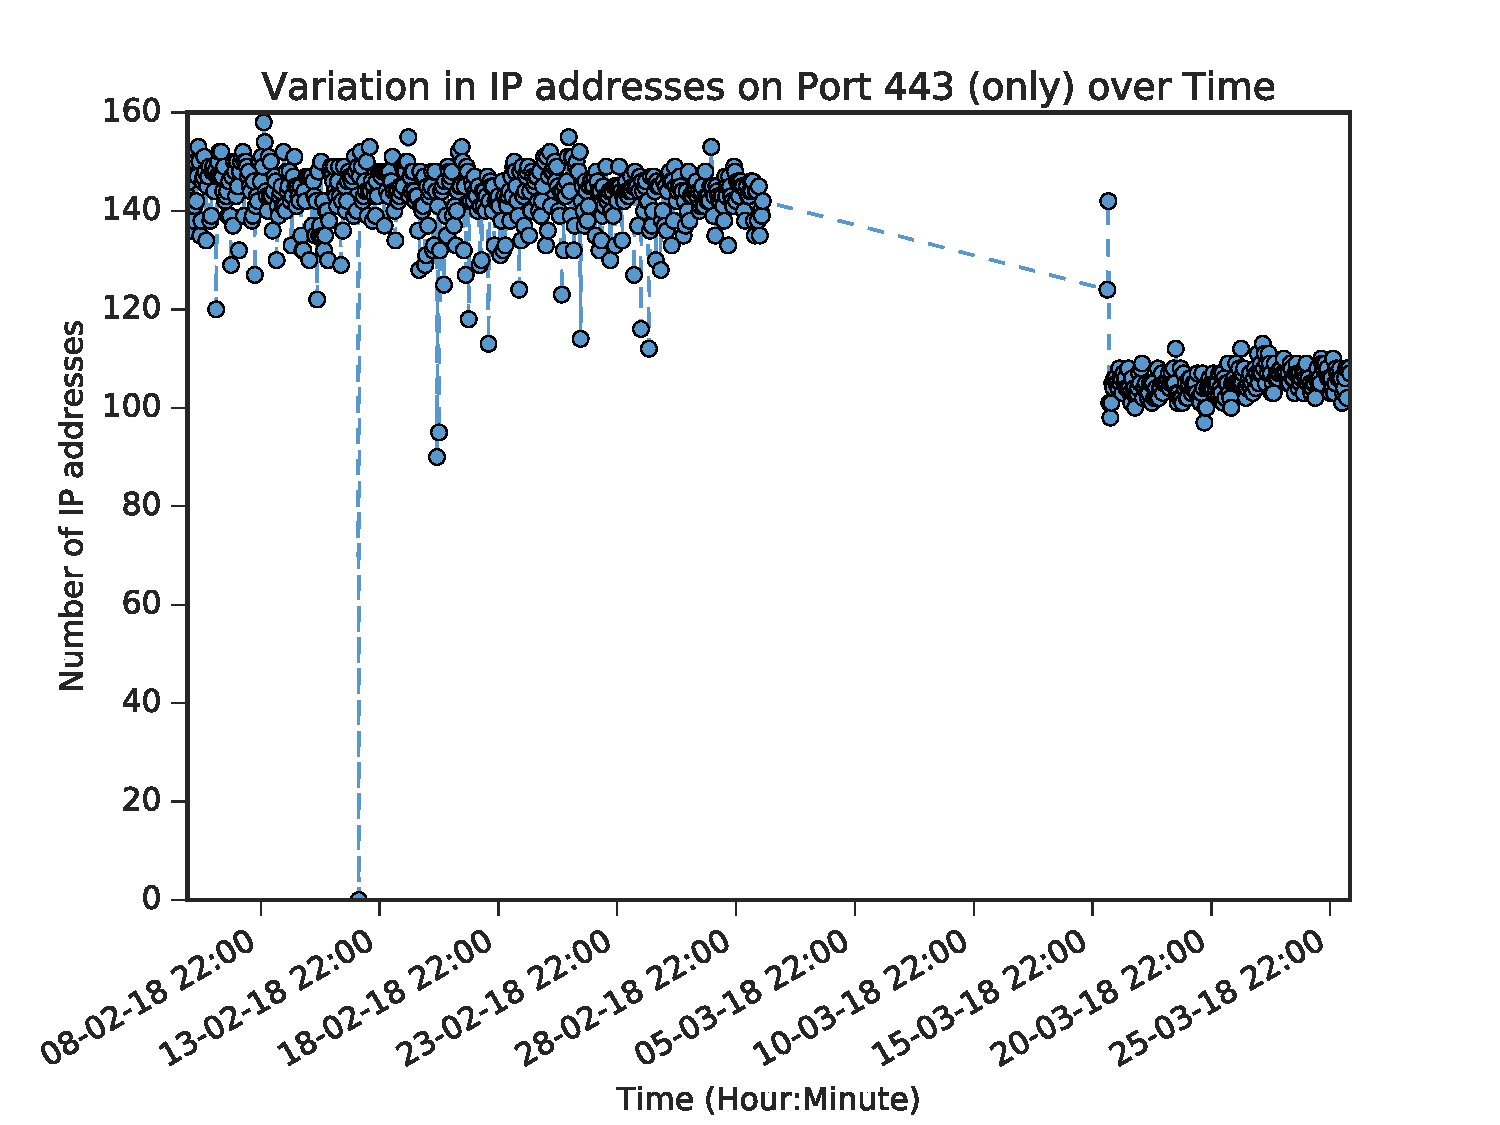
\includegraphics[scale=.5]{pdf_images/VariationInIpAddressesOnPort443OverTime}
\caption{a nice plot1}
\label{fig:port443ZMap}
\end{figure}



From figure \ref{fig:port443ZMap} we can see the failed scan that appeared on the 13th of Feburary at 1am which lead to the overly high count of IP addresses on port 80 (only) for this observational slice.

Another interesting incident that was observed is the drop in the average number of IP addresses from 145 before the server was cut off to to 105 after the server was back up and running.

\begin{figure}[h!]
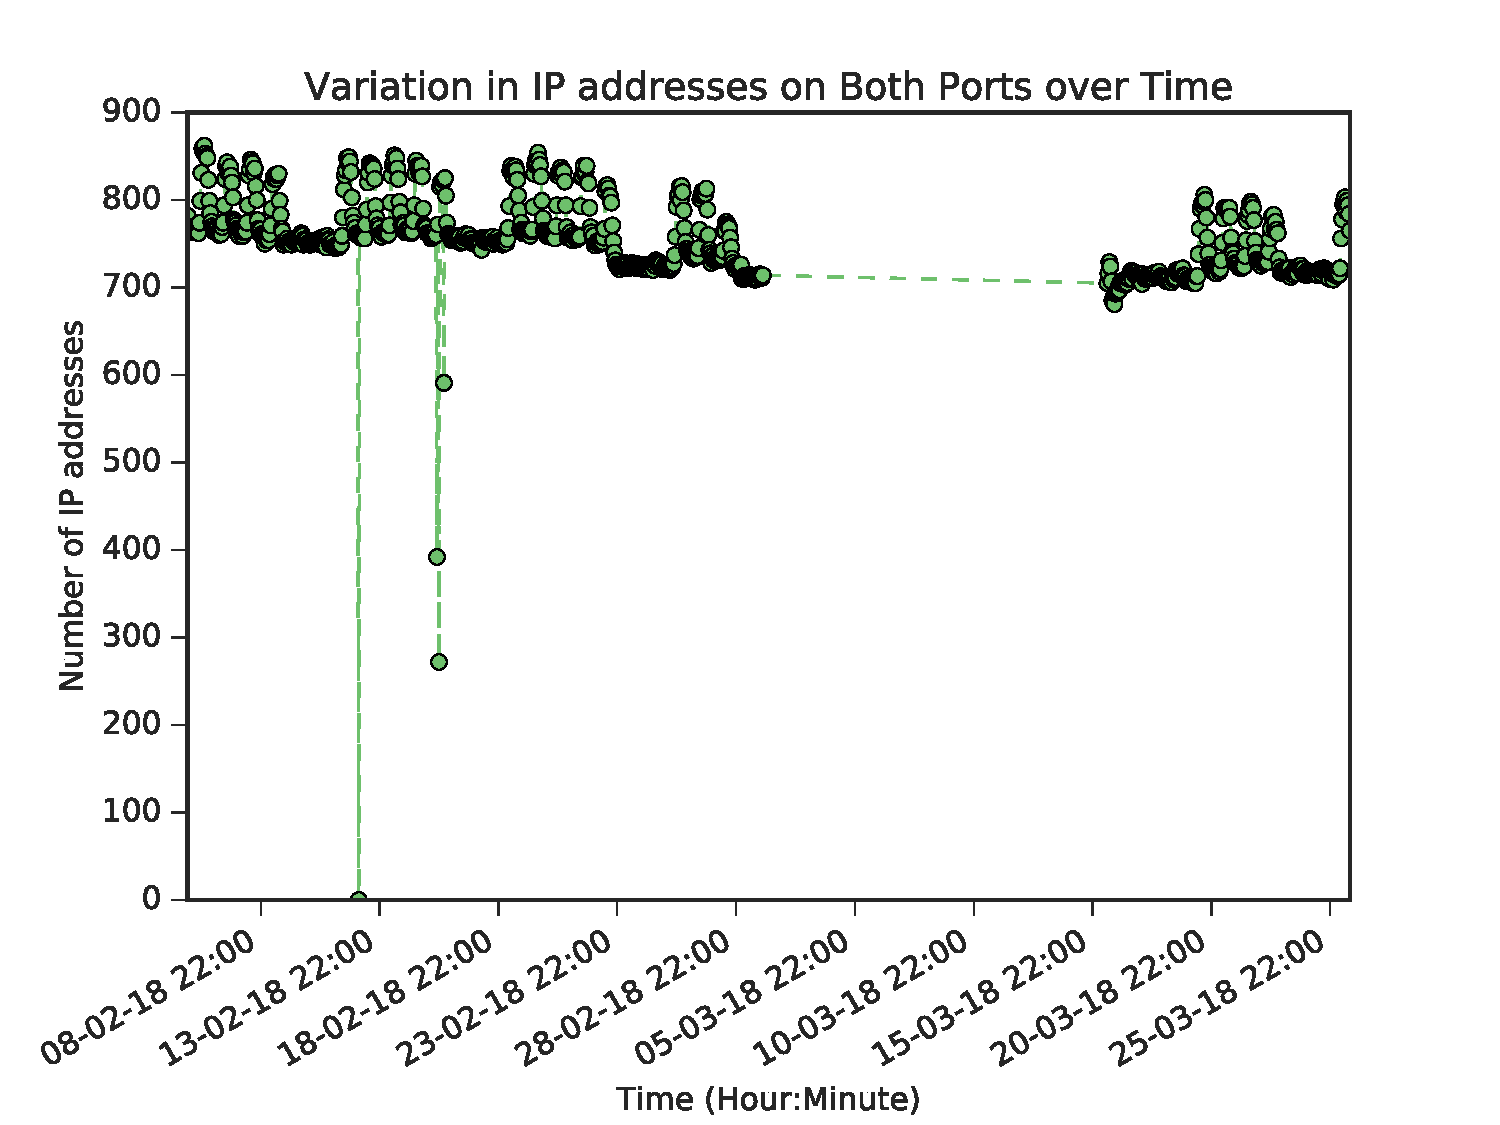
\includegraphics[scale=.5]{pdf_images/VariationInIpAddressesOnBothPortsOverTime}
\caption{a nice plot1}
\label{fig:portsBothZMap}
\end{figure}
From figure \ref{fig:portsBothZMap} we can see a similar trend that was observed in the figure \ref{fig:port80ZMap} with a higher number of IP addresses being present throughout the weekday and falling at the weekend.\\

There is also no dramatic change in the average number of IP addresses being present before and after the server cut off that was seen in figure \ref{fig:port443ZMap}


\begin{figure}[h!]
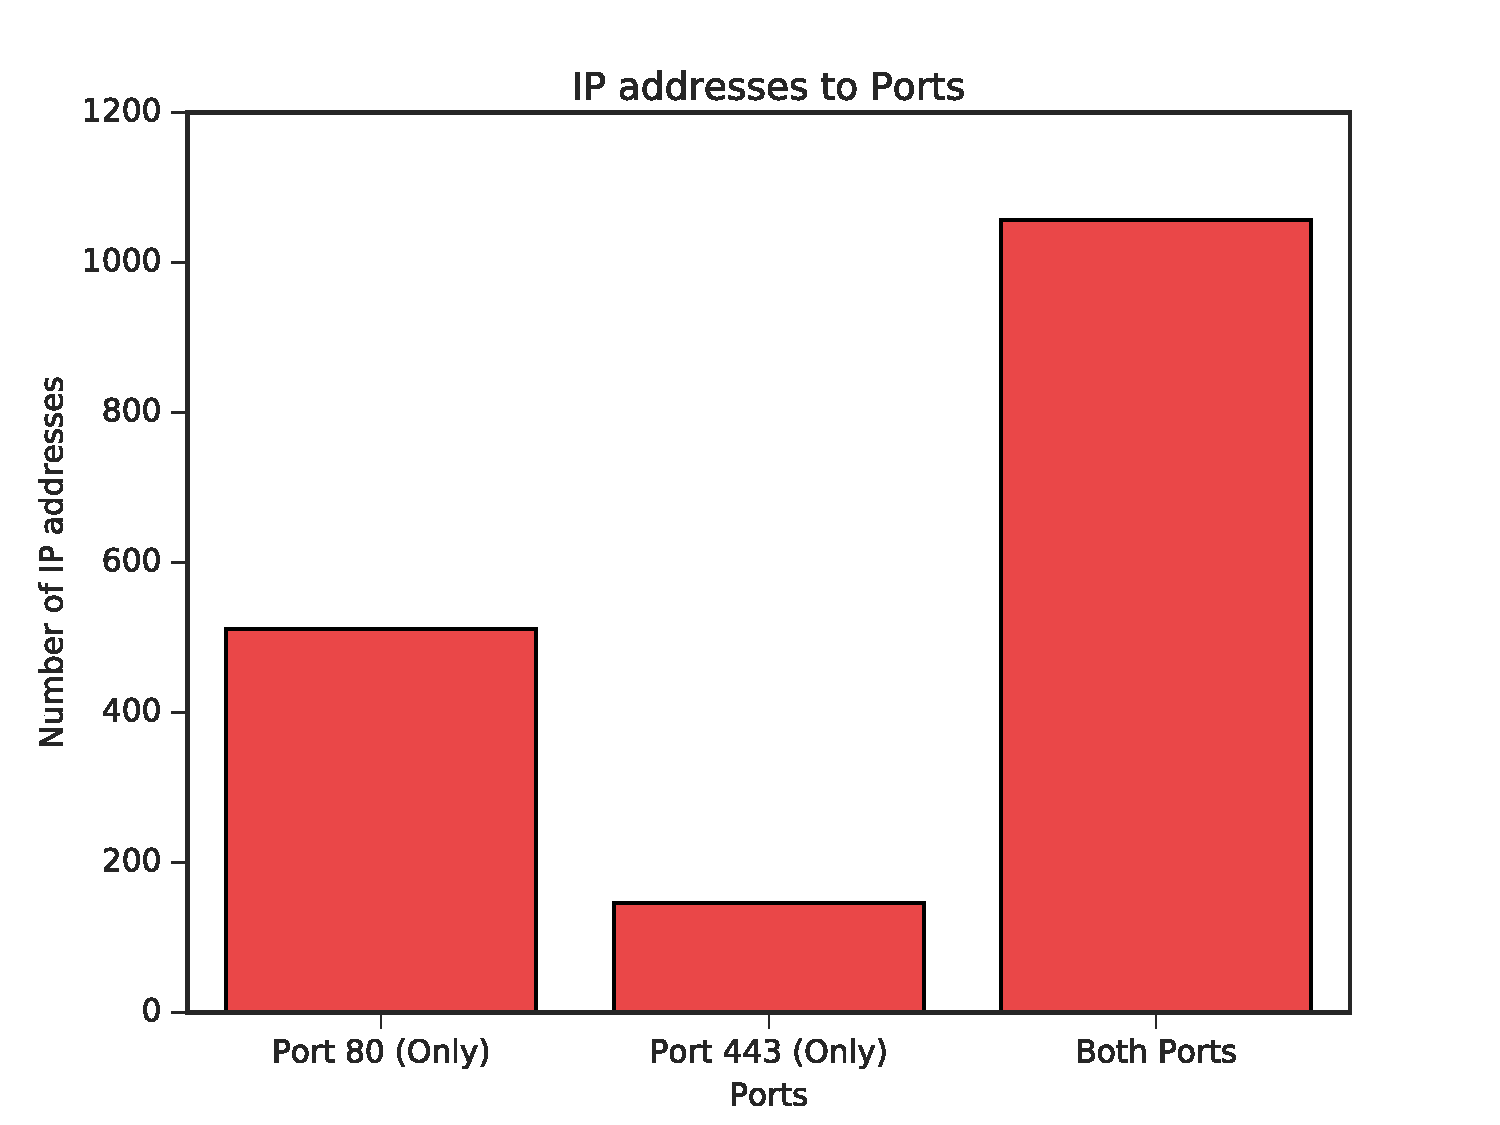
\includegraphics[scale=.5]{pdf_images/IPaddressestoPorts}
\caption{a nice plot1}
\label{fig:ports}
\end{figure}
In all there was a total of 1714 unique IP addresses that were seen throughout the ZMap scans, from figure \ref{fig:ports} we can see a breakdown of the 3 main categories of IP addresses Port 80 (only) which are IP addresses that are were only observed on Port 80 and no other port, Port 443 which were IP addresses only observed on Port 443 and no other port, and finally Both Ports which consisted of IP addresses that were on both Port 80 and 443 at some point throughout the ZMap scans.\\

We recorded 511 IP addresses on port 80 alone, followed by 146 IP addresses on port 443 and lastly 1057 IP addresses on Both ports.

\begin{figure}[h!]
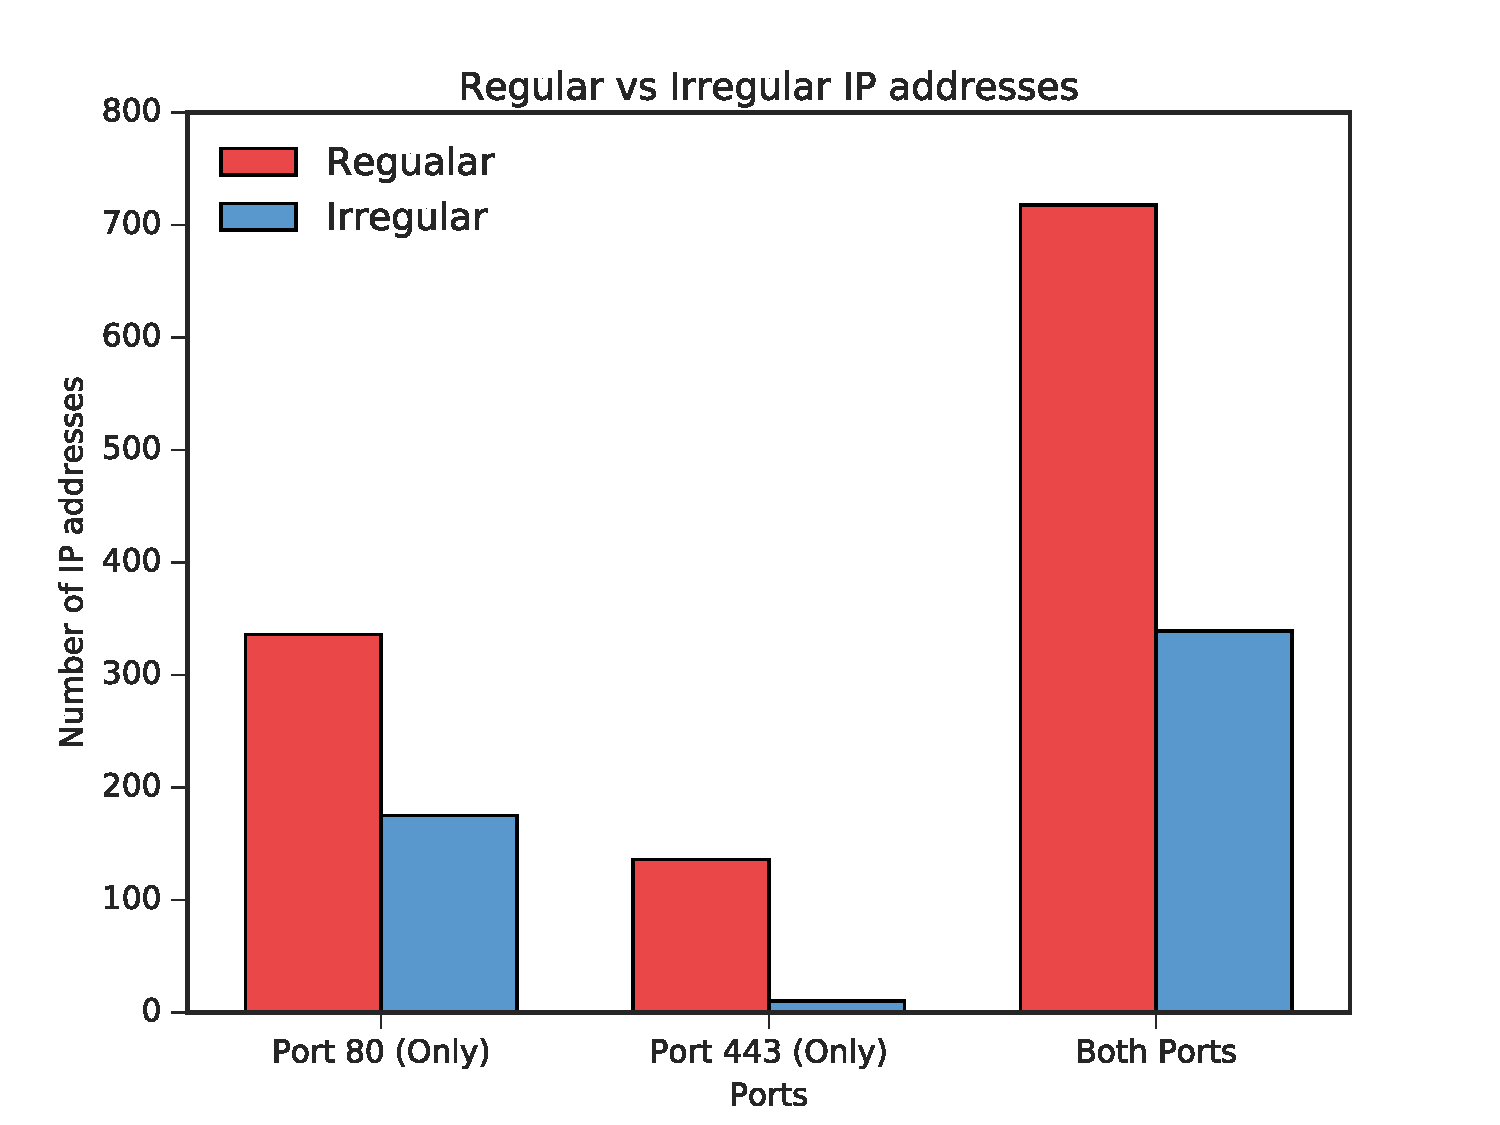
\includegraphics[scale=.5]{pdf_images/RegularVsIrregularIPaddresses}
\caption{a nice plot1}
\label{fig:portsIrreg}
\end{figure}

From the scans (figure \ref{fig:average_day}) we noticed a number of irregularities in terms of the number of IP addresses that would be up at any given hour, to investigate this aspect of the data we decided to filter the IP addresses in terms of those that are regular which in our case is
IP addresses that are seen 90\% of the time which is 744 from 827 observational slots. Everything else is consider an Irregular IP address.

The above figure \ref{fig:portsIrreg} shows the comparison between each port category, with a total of 1190 IP addresses being Regular with 336 being on Port 80 (only), 136 on Port 443 (only) and 718 being on Both Ports. Similarly we observed that 524 of the total IP addresses observed in the scans are Irregular, with 175 of those being on Port 80 (only), 10 being on Port 443 (only) and 339 on Both Ports.


\begin{figure}[h!]
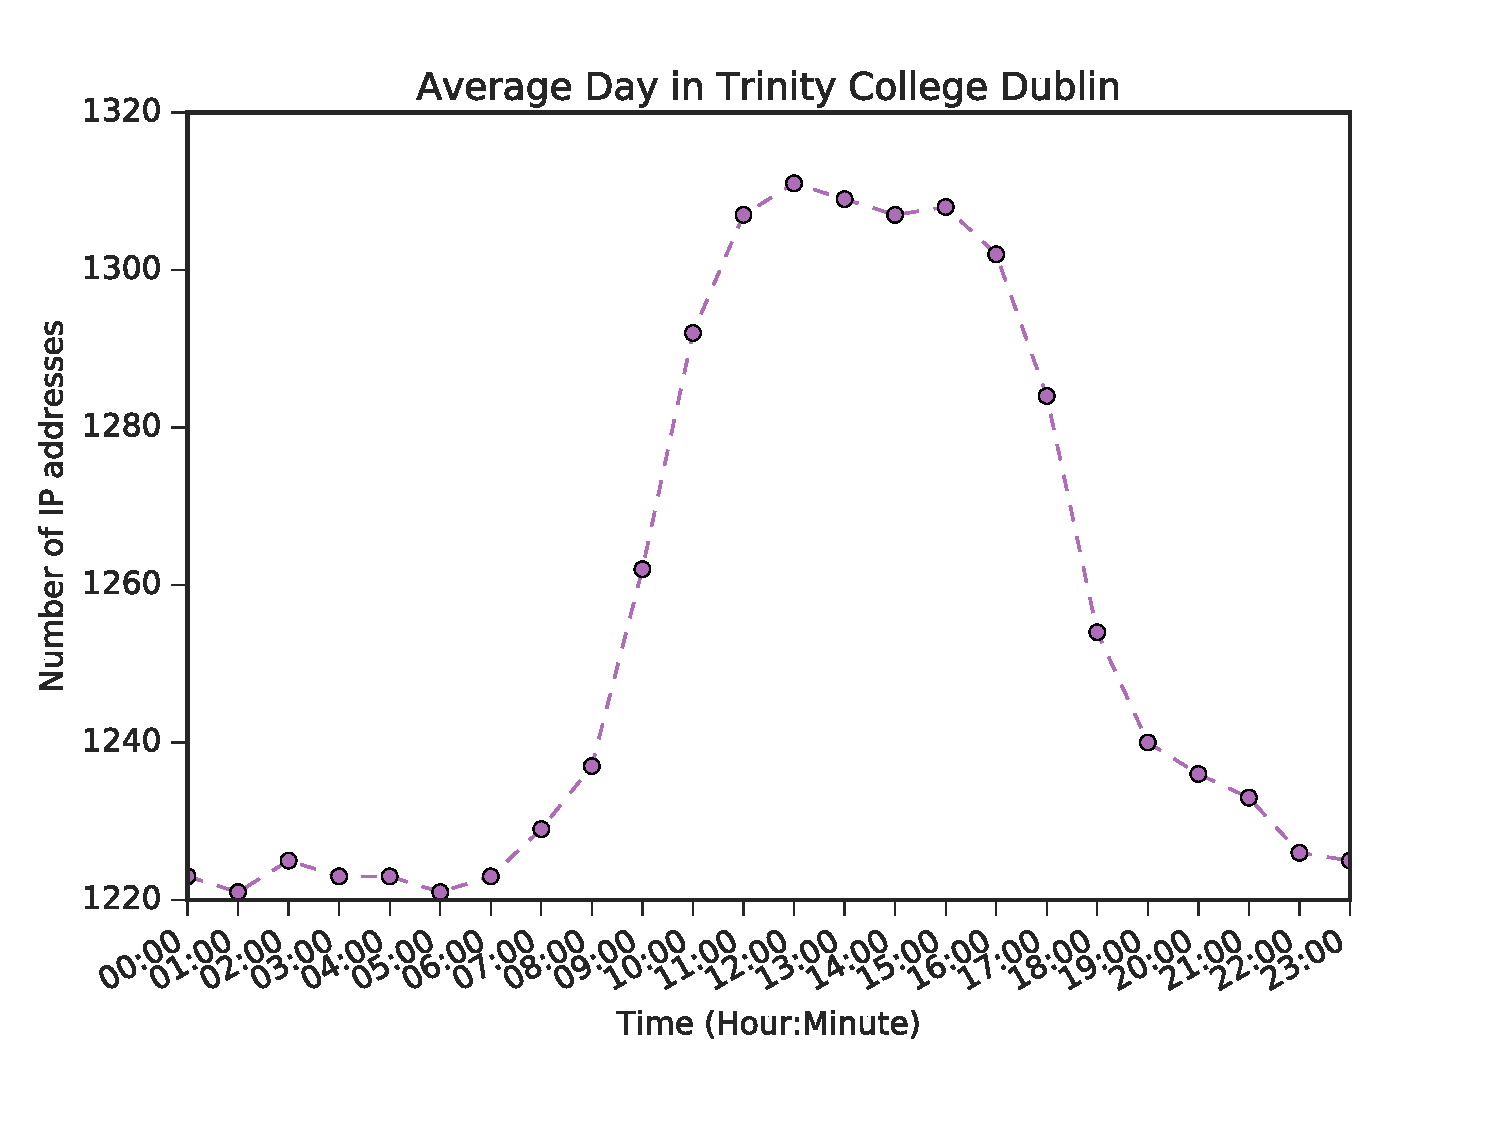
\includegraphics[scale=.5]{pdf_images/AverageDayinTrinityCollegeDublin}
\caption{a nice plot1}
\label{fig:average_day}
\end{figure}
When looking at all the IP addresses on average over a 24 hour period as we can see in figure \ref{fig:average_day} there is a large count of IP addresses between 11am to 4pm

Peak time on Average in the college is 12pm midday with 1311 IP addresses being present
Off-Peak time are 1 am and 5 am with both counting 1221 IP addresses being present.

\begin{figure}[h!]
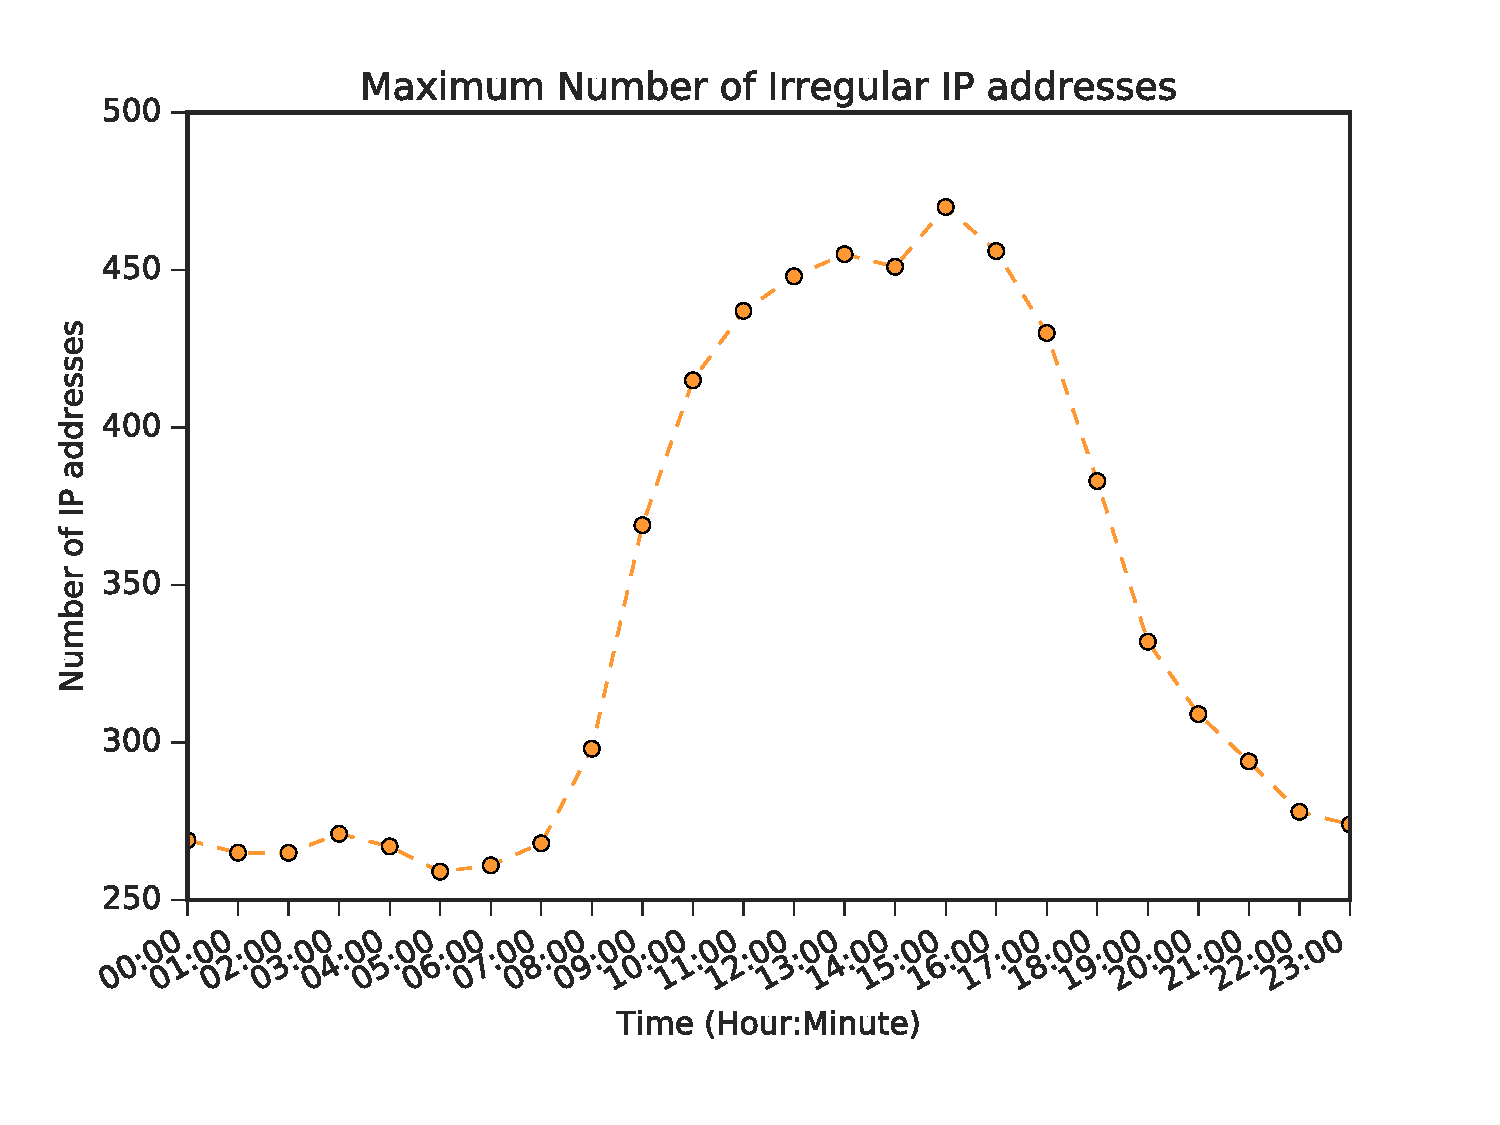
\includegraphics[scale=.5]{pdf_images/MaximumNumberOfIrregularIPaddressesInAnAverageDay}
\caption{a nice plot1}
\label{fig:irreg_ips}
\end{figure}
When analysing the hour that an Irregular IP address has ever been on such as in figure \ref{fig:irreg_ips} we see that at some point over the time of the scans particularly at 3pm there has been 470 of the 524 Irregular IP addresses active at this hour throughout the ZMap scans. On the opposite scale 259 IP addresses have be present at 5am at some point in time over the series of scans conducted. This might lead us to believe that the majority of Irregular IP address occurs at 5pm which is not the case when we look at the individual occurrences in figure \ref{fig:irreg_occurence}.

\begin{figure}[h!]
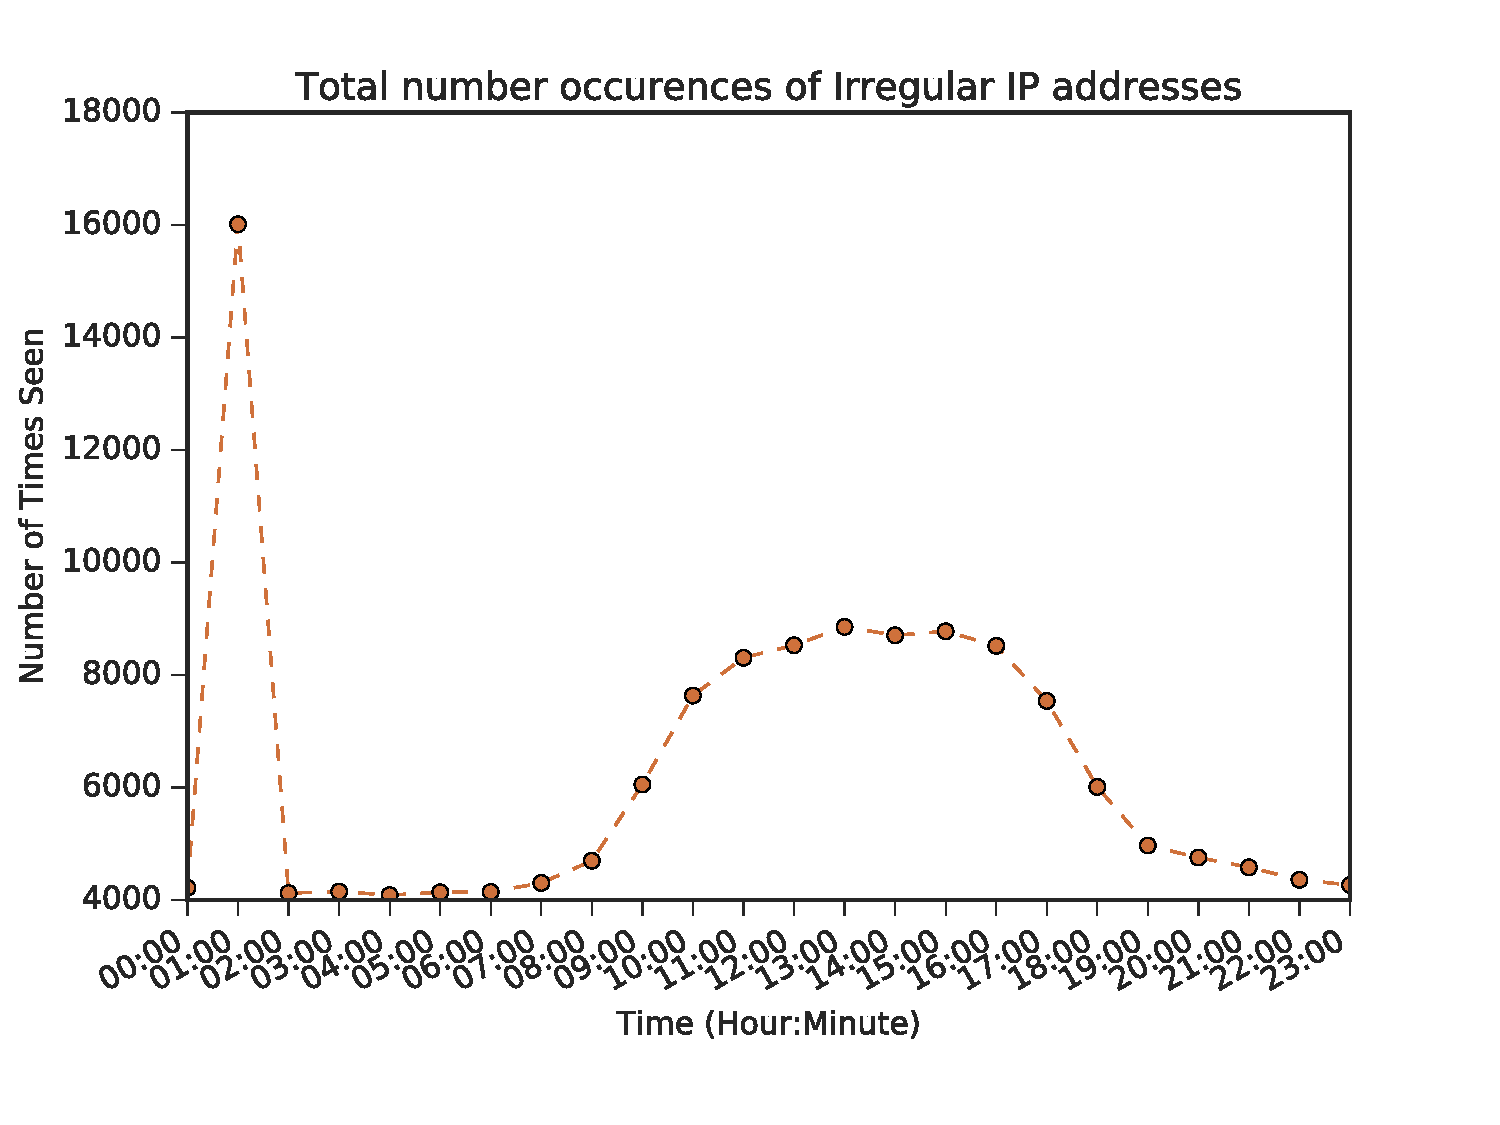
\includegraphics[scale=.5]{pdf_images/TotalNumberOccurencesOfIrregularIPaddressesOnAverage}
\caption{a nice plot1}
\label{fig:irreg_occurence}
\end{figure}
When counting each occurence of an IP address on either port we see in figure \ref{fig:irreg_occurence} that there is a large discrepancy between the number of occurrence of an IP and the hour that each IP appears. For example we see in figure \ref{fig:irreg_occurence} that the number of occurrences that happen at 1am is 16014 where as at 3pm, 8777 occurrences have taken place throughout the ZMap scanning period which is the second largest number of occurrences. This large difference on further inspection of the data is due to 27 Unique IP address of which only 10 were on port 80 (only), 1 on port 443 (only) and 16 on both ports.



\begin{table}
\centering
\begin{tabular}{|| c c ||}
 \hline
  Total Occurrences & Occurrences at 1am  \\ [0.5ex]
 \hline\hline
 1520 & 720  \\
 1496 & 720 \\
 1354 & 716 \\
 1294 & 710  \\
 1444 & 710 \\
 1159 & 702 \\
 1018 & 698 \\
 729 & 688  \\
 1633 & 390 \\
 1446 & 388 \\[1ex]
 \hline
\end{tabular}
\caption{Top 10 Irregular IP addresses seen at 1am }
\label{table:2}
\end{table}

From figure \ref{table:2} we can see that the vast majority of occurrences at 1am account for a major period of the overall number of occurrences. of these 27 that cause this large difference, 17 of them have 50\% or greater with the number of occurrences that are seen at 1am compared to every other day in the week combined.
 

!!!!!!!!!!!!!!!!!!!!!!RE DO IPS TO HOSTNAME PIECHART !!!!!!!!!!!!!!!!!!!!
\begin{figure}[h!]
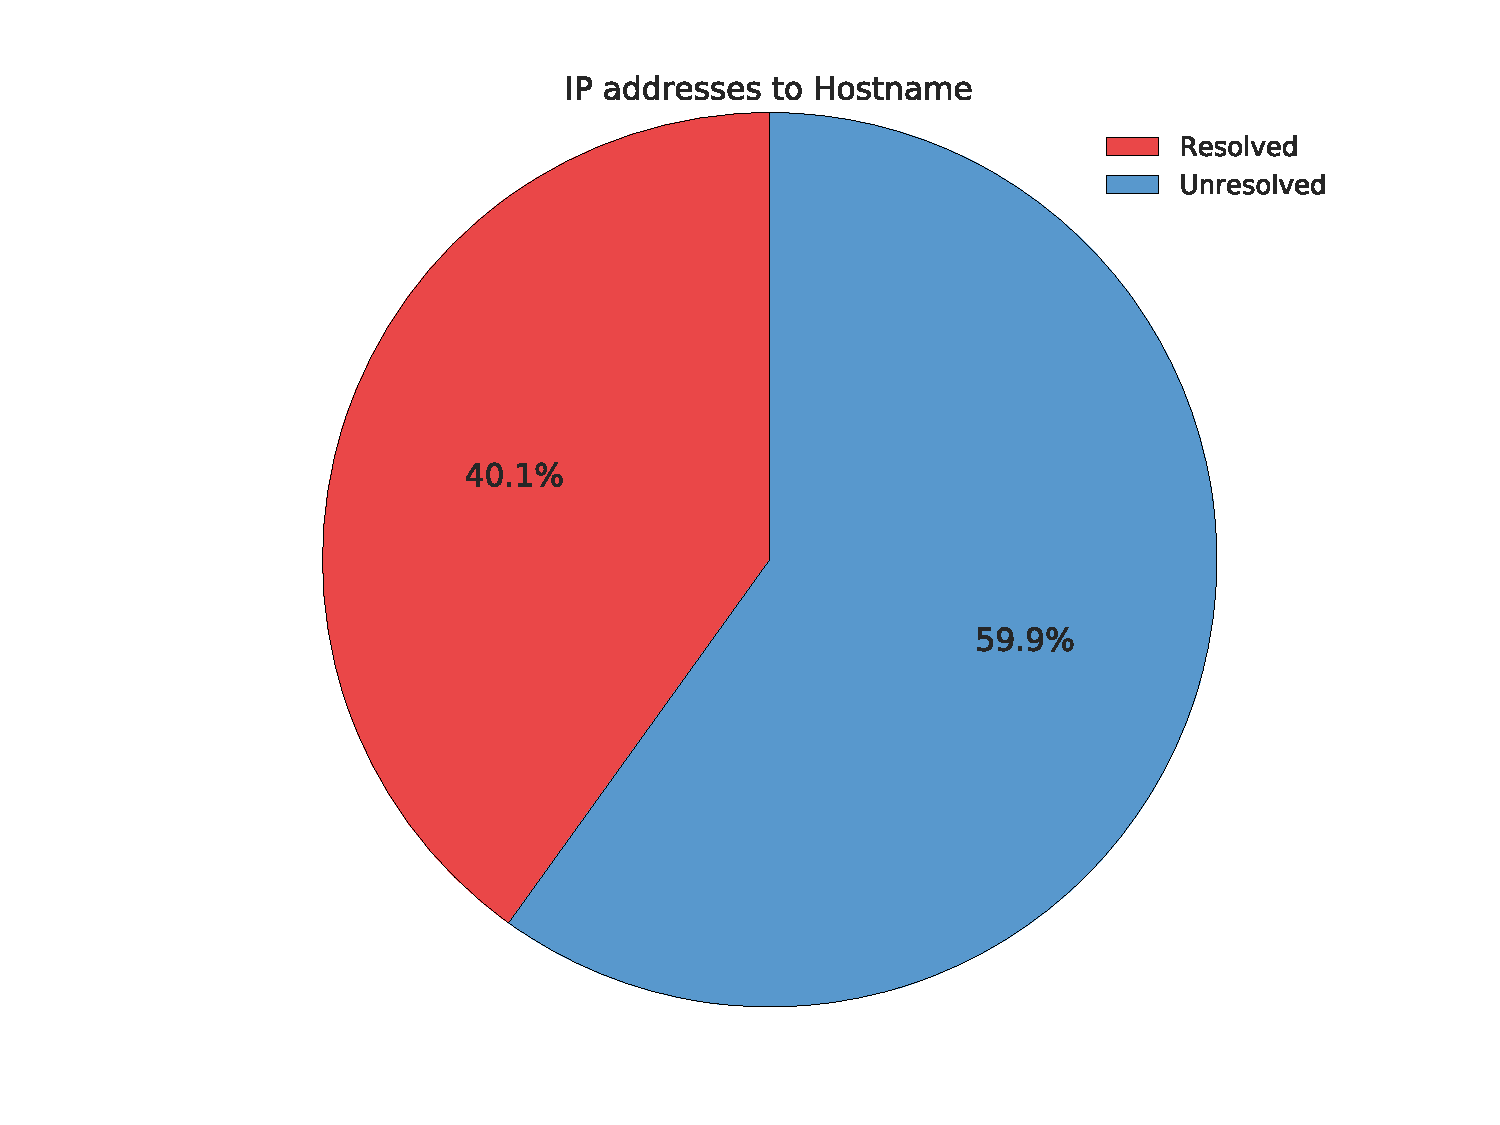
\includegraphics[scale=.5]{pdf_images/IpstoHostname}

\end{figure}
\section{ZGrab Results}
\begin{figure}[h!]
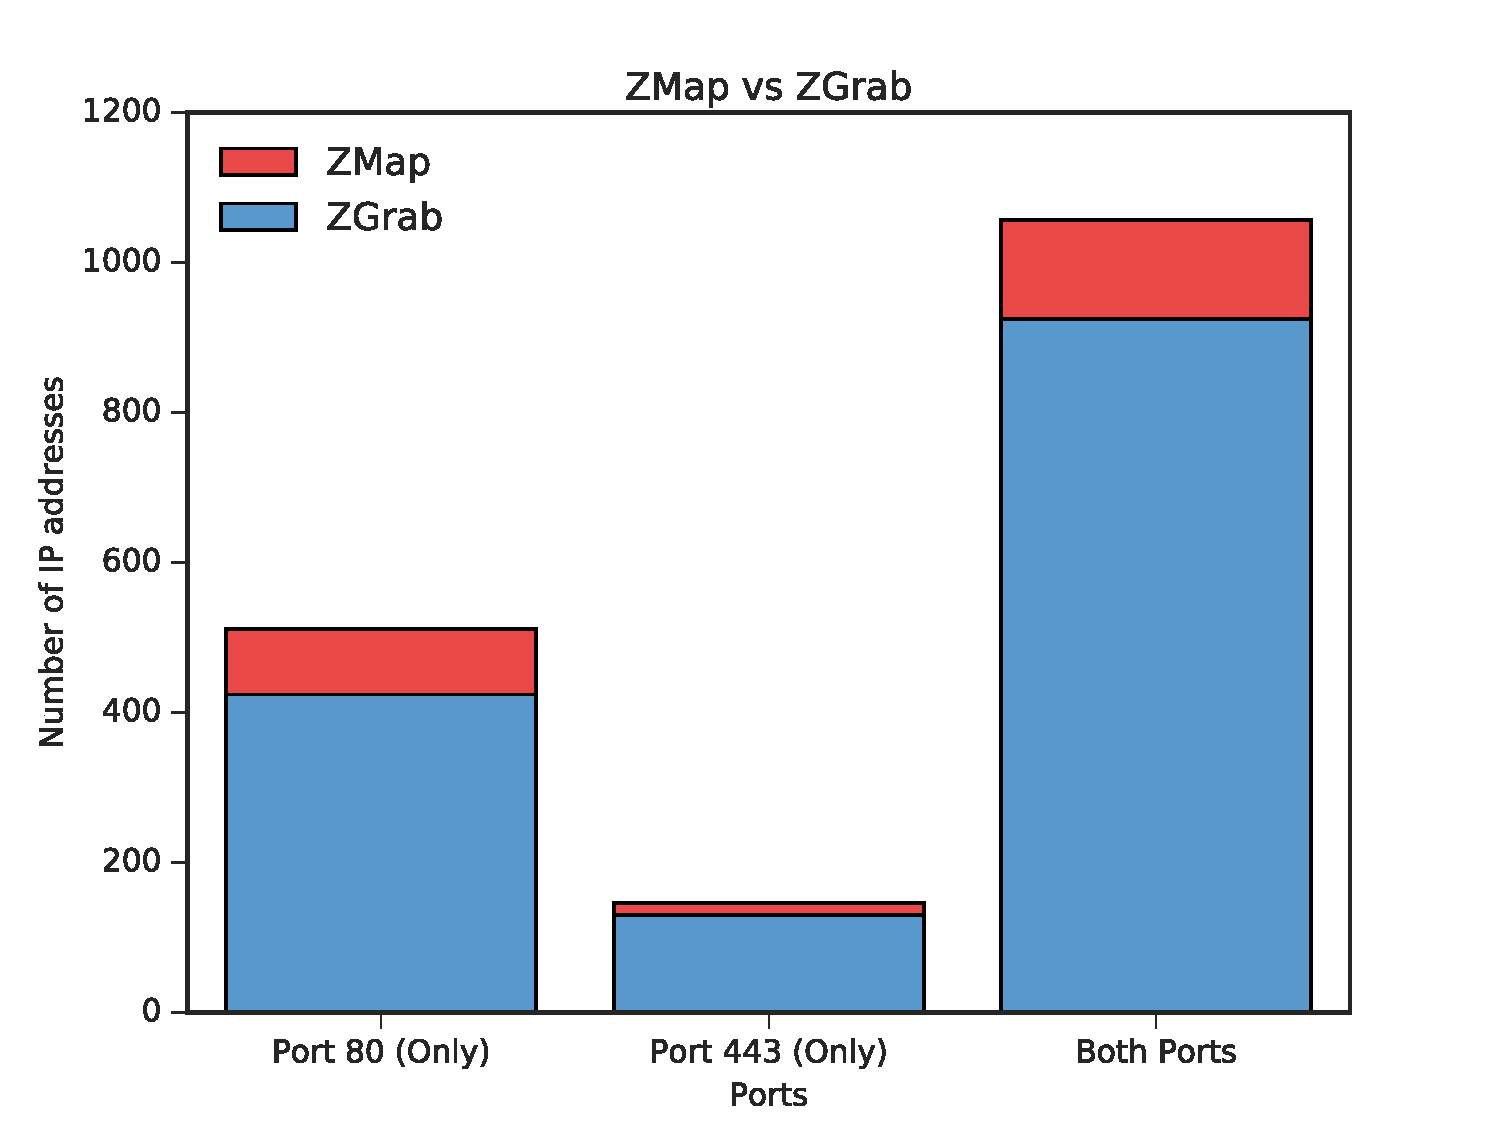
\includegraphics[scale=.5]{pdf_images/ZMapVsZGrab}
\end{figure}

!!!!!!!!!!!!!!!!!!!!! MIGHT HAVE TO REDO GRAPH ABOVE !!!!!!!!!!!!!!\\



\begin{figure}[h!]
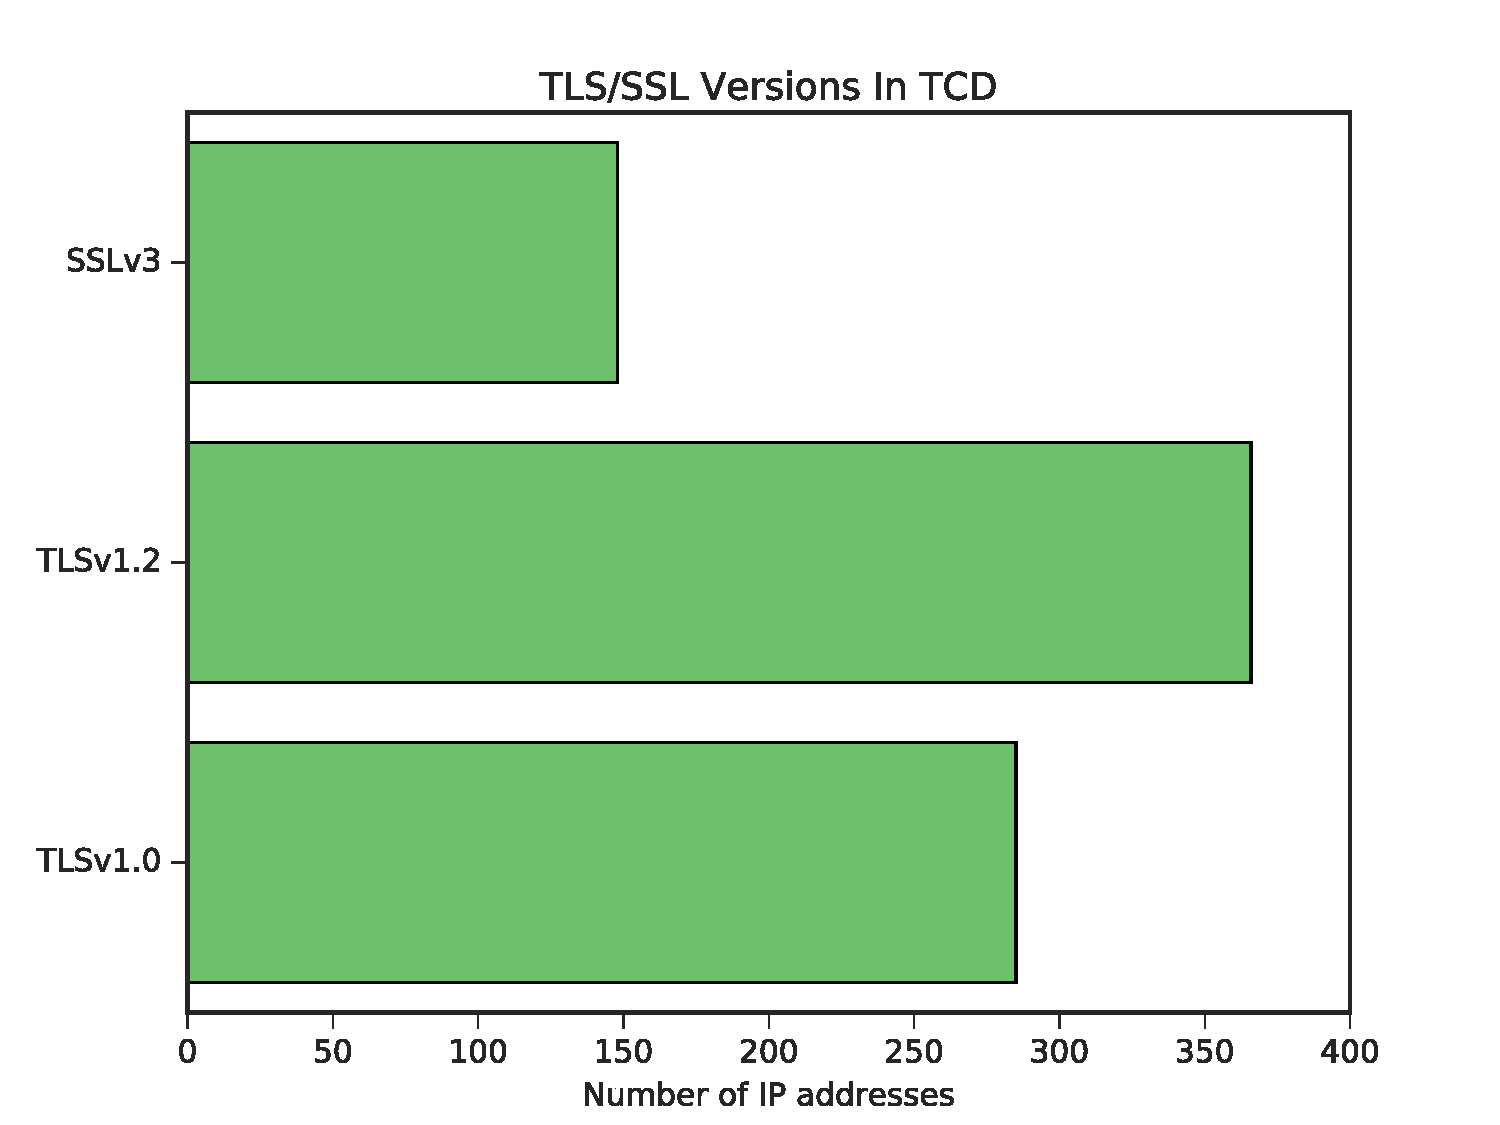
\includegraphics[scale=.5]{pdf_images/TLSVersionsInTCD}
\caption{a nice plot1}
\label{fig:TLS_SSL}
\end{figure}

Over the course of the banner grabs we have found 3 different versions of TLS/SSL being implemented in the college to provide encryption of data. It turns out that SSL 3.0 is still being used despite the fact that it is inherently broken and suffers from various attacks such as POODLE\cite{holz2015summarizing} \cite{moller2014poodle} and many organisations \cite{ssllabs} advise not to use it  but use TLSv1.2 instead. One of the reasons as to why this old implementation of SSL/TLS is still being used, might be the fact that many legacy web browser such as IE6/XP only support SSL 3.0 and thus switching off support for SSL 3.0 would prevent browsers from working with the site \cite{owaspTLS_SSL}. Next we have TLSv1.0 which is the next version of TLS after SSLv3.0, similar advise is given with regards to the use of TLSv1.0 as it too is also a legacy protocol that suffers from problems such as the BEAST attack\cite{holz2015summarizing} which is an vulnerability in the implementation of the Cipher Block Chaining (CBC) in TLSv1.0. The most secure of the TLS versions found in the college has the greatest number of IP addresses (366) that are using it, to secure their communication. No version of TLS1.1 was ever discovered throughout the ZGrabs.


\begin{figure}[h!]
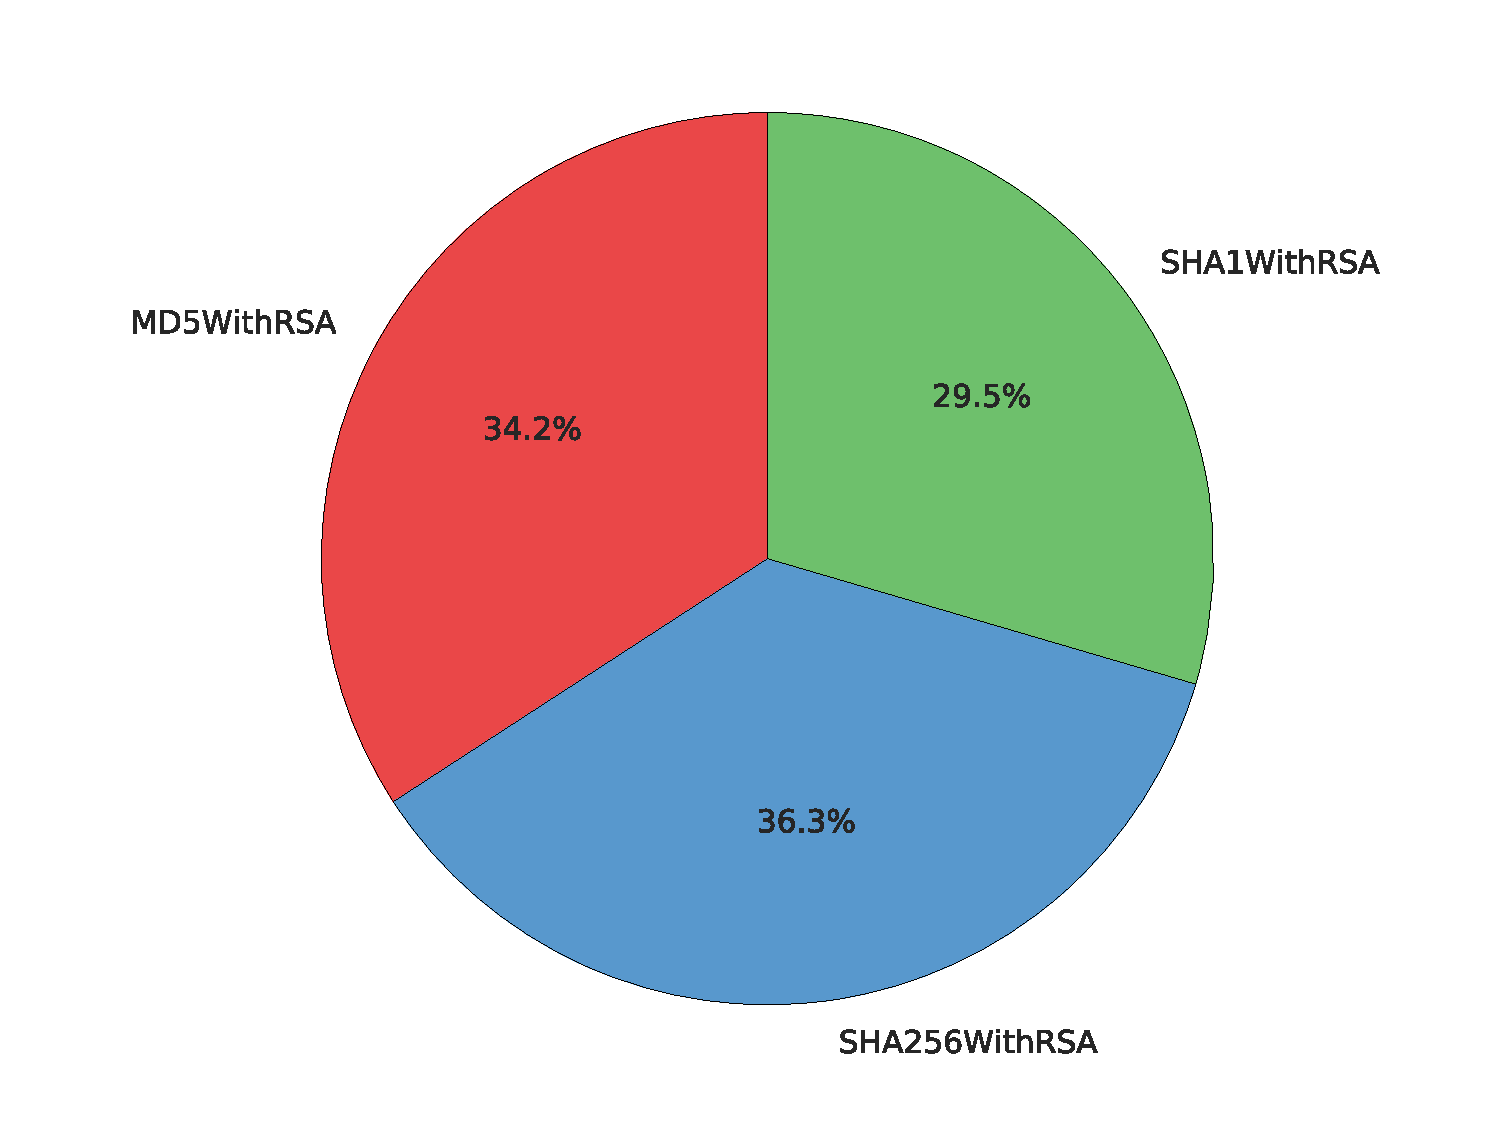
\includegraphics[scale=.5]{pdf_images/signatureAlgorithms}
\caption{a nice plot1}
\label{fig:signatureAlgorithms}
\end{figure}

One of the more surprising discoveries is the prevalence of MD5 hash function. In total we found 273 unique IP addresses that are using MD5withRSA to sign their certificates. According to the Internet Engineering Task Force MD5 is no longer acceptable where collision resistance is required
such as digital signatures \cite{turner2011updated} this is due to the fact that MD5 hash functions allows the construction of different messages with the same MD5 hash resulting in a collision \cite{md5}. Along with MD5 being fundamental broken, SHA1 is also now insecure. Both of these signature algorithms in figure \ref{fig:signatureAlgorithms} used to sign certificates account for 63.7\% of 799 IP addresses in the college using unsecured hashing functions.\cite{ssllabs}. With the remaining 290 IP addresses possessing certificates signed with SHA256 which is the recommend signature algorithm to use\cite{ssllabs}.

\begin{figure}[h!]
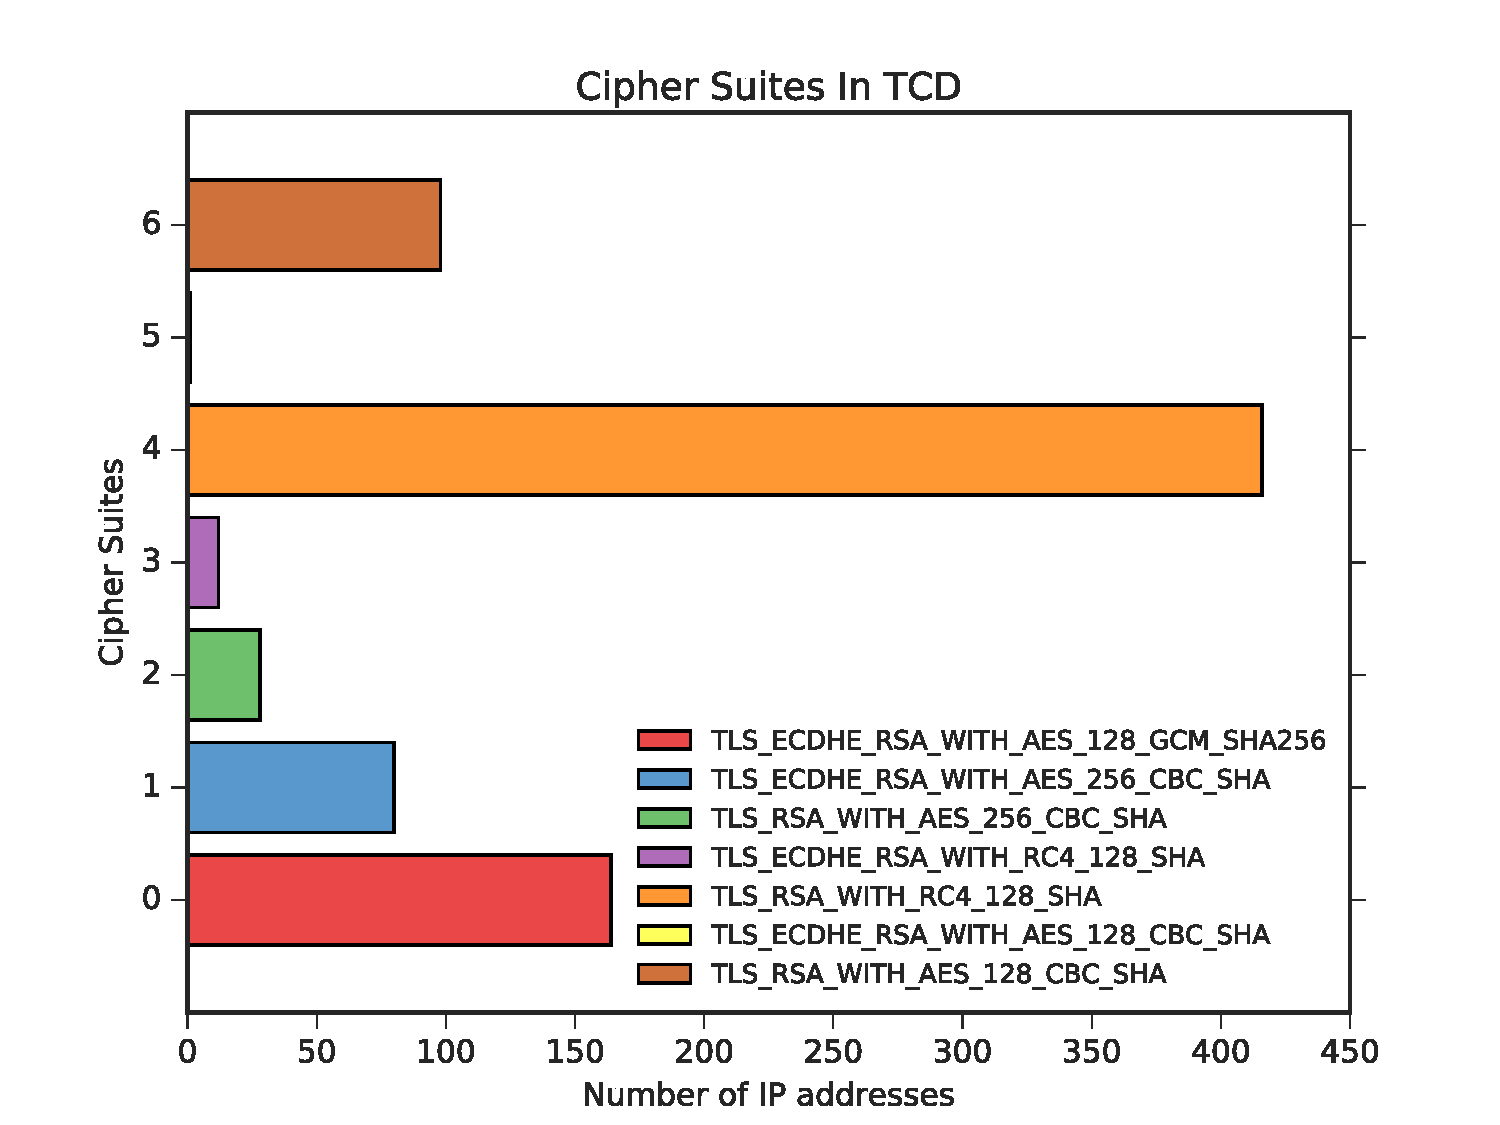
\includegraphics[scale=.5]{pdf_images/CipherSuitesInTCD}
\caption{a nice plot1}
\label{fig:cipherSuites}
\end{figure}

As we can see in figure \ref{fig:cipherSuites} $TLS_RSA_WITH_RC4_128_SHA$ is by far the most widely used cipher suite in the college, even though community at large advise against RC4 cipher suites as the bytes used to encrypt plaintext is not as random as one would hope resulting in attackers being able to exploit the bias in the keystream that encrypyt the plaintext, uncovering previous encrypted plaintext messages \cite{popov2015prohibiting}. The most least wide cipher suite found is  $TLS_ECDHE_RSA_WITH_AES_128_CBC_SHA$ with only a single IP address offering up this in cipher suite to be used.

\begin{figure}[h!]
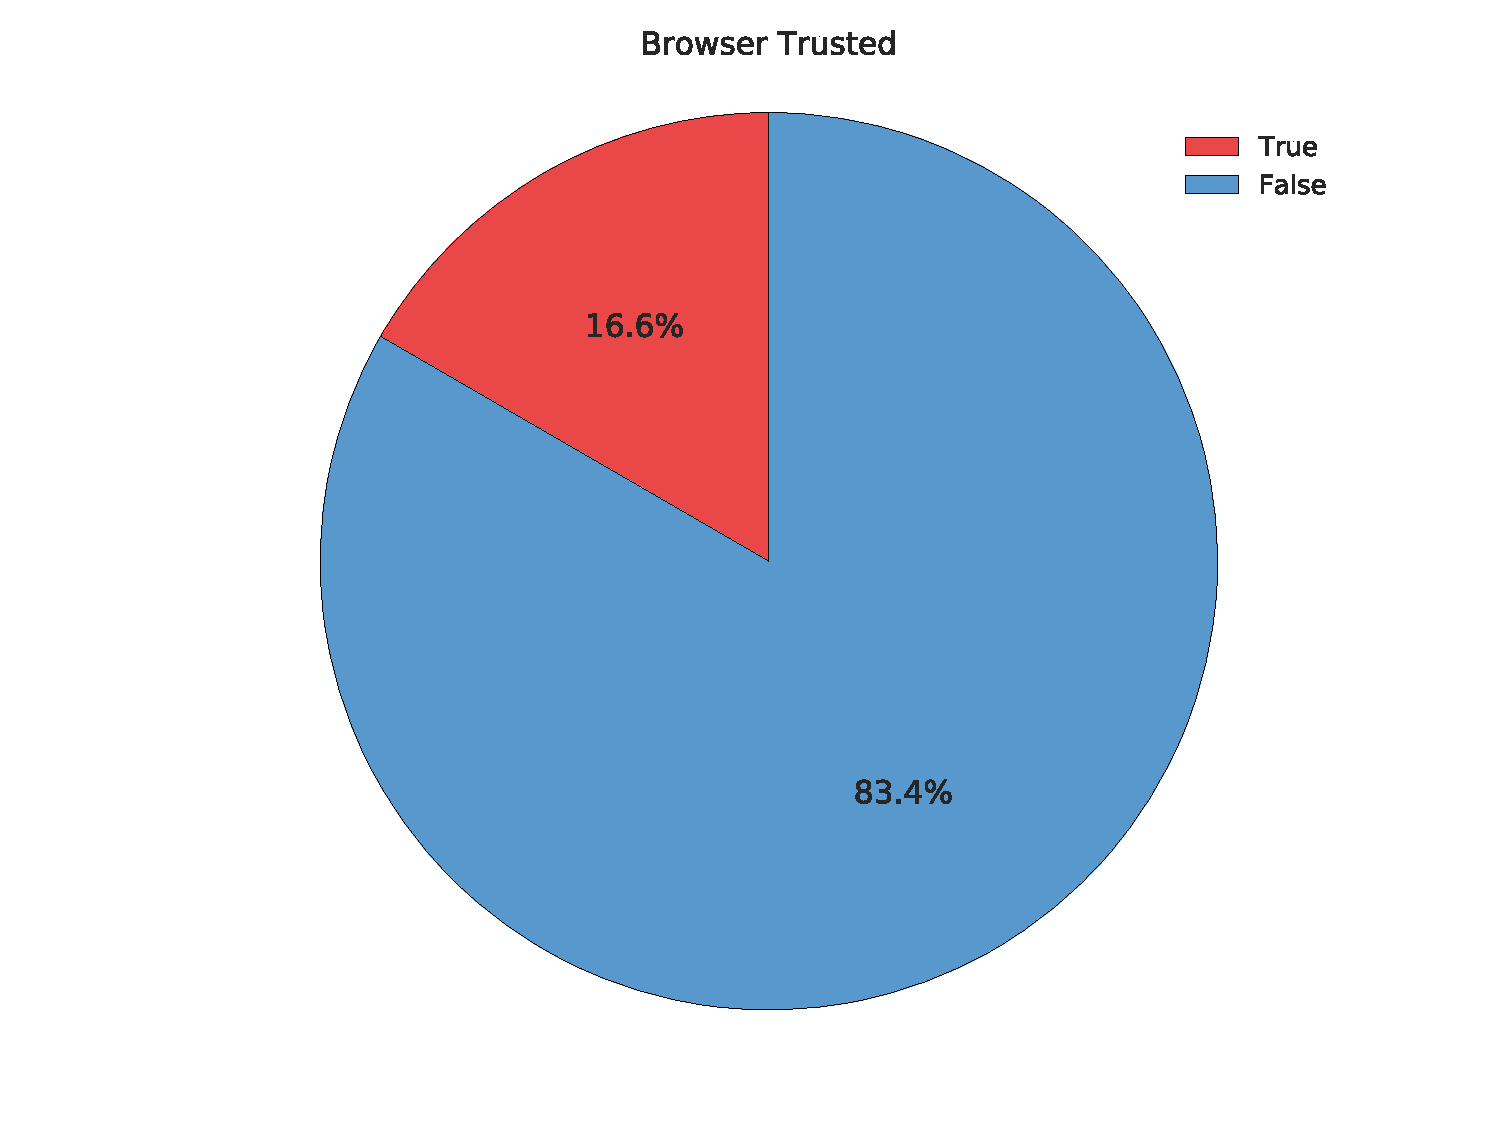
\includegraphics[scale=.5]{pdf_images/BrowserTrusted}
\caption{a nice plot1}
\label{fig:browserTrusted}
\end{figure}
Of the certificates we managed to collect only 133 were browser trusted. Further more the cipher suites that browser trusted certificates use differs from that of the entire certificates collected with 45 IP address of using  $TLS_ECDHE_RSA_WITH_AES_128_GCM_SHA256$ cipher suites and only 17 using $TLS_RSA_WITH_RC4_128_SHA$. All the browser trusted certificates have been found to use SHA256withRSA as any certificate signed with MD5 or SHA1 is considered insecure \cite{ssllabs}.
 


\begin{figure}[h!]
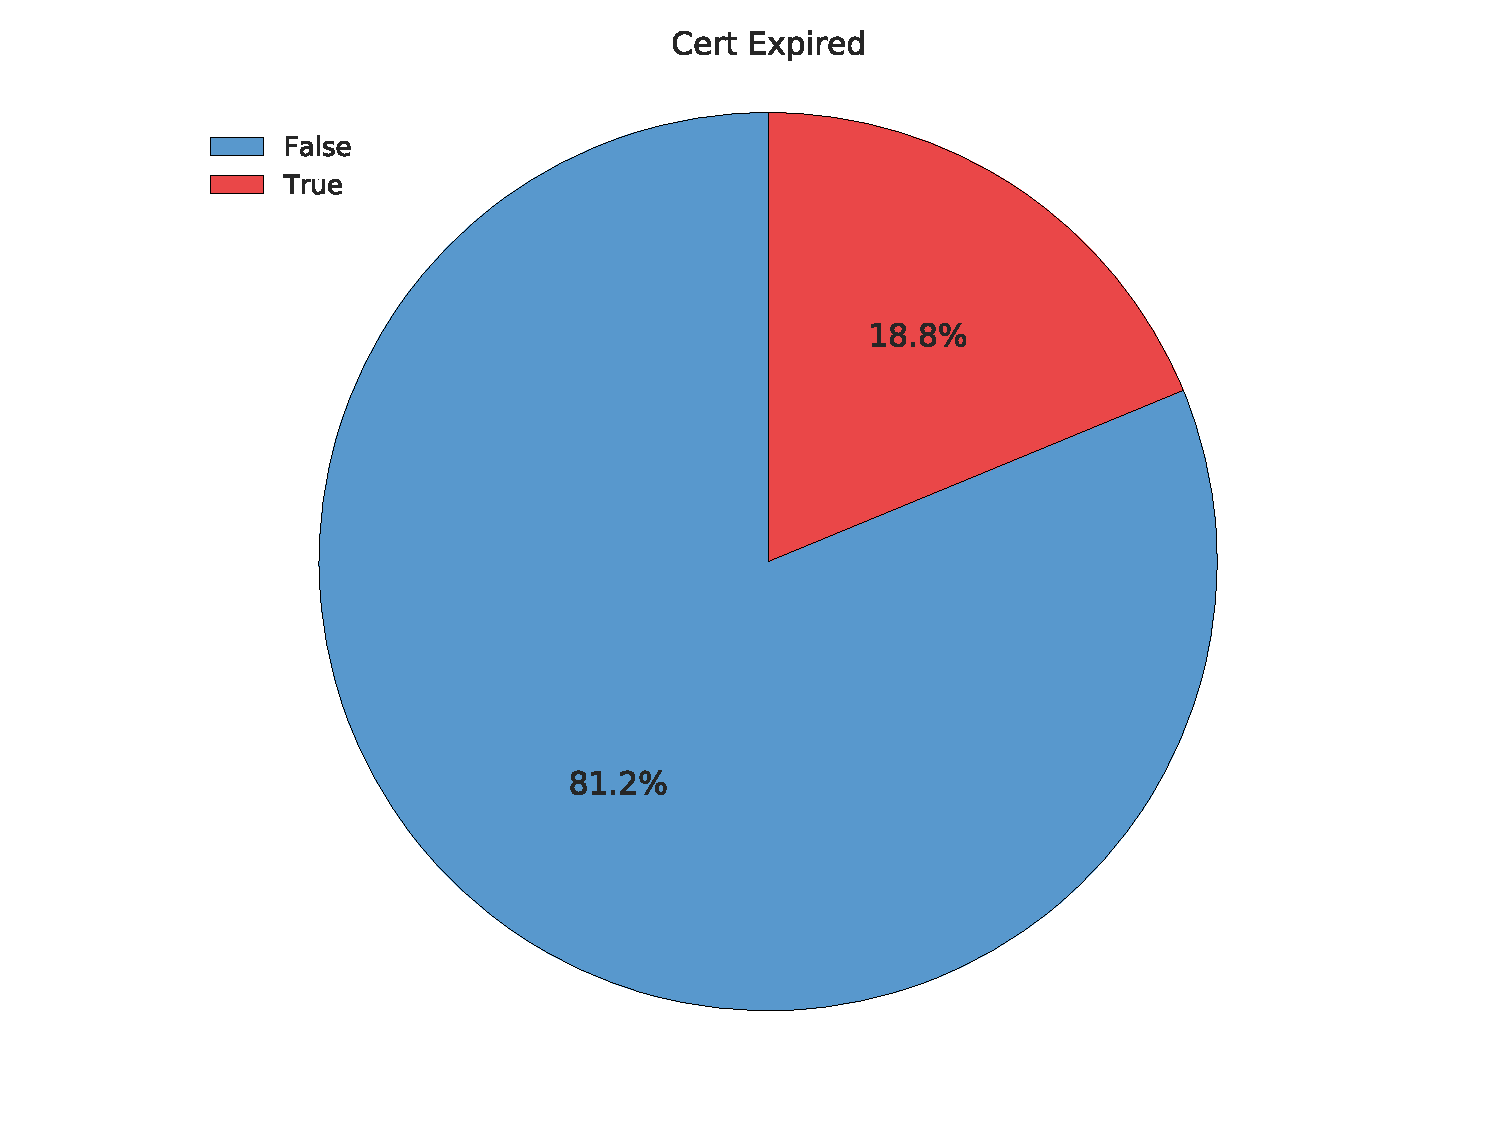
\includegraphics[scale=.5]{pdf_images/CertificateExpired}
\caption{a nice plot1}
\label{fig:certExpired}
\end{figure}

From figure \ref{fig:certExpired} we can see that 18.8\% which is 150 IP addresses have certificates that are out of date.



\chapter{Conclusion}
\cite{turner2014transport} page 62,63

\cite{mendes2008assessing} page 316
\chapter{Future Work}
Would be beneficial if we could find out the total number of host on port 80 and port 443 from system admins to determine whether or not the scans detecting all host on port 80 and port 443 in order to judge the successfulness of ZMap\\

Looking at the adoption rate of protocols within the college similarly done by \cite{durumeric2013zmap} page 9 and \cite{durumeric2013analysis} page 11.\\

Talk about what I have done could be used as a infrastructure in order for other universities to survey their own web servers as well as maybe having the ability to automate it with alerts being sent out if a certain type of cipher suite is found or old version of TLS is discovered\cite{durumeric2015search} page 5 talks about something similar\\

Scanning IPv6 address space within the college \cite{durumeric2013zmap} page 14\\

Investigate the detection capabilities of ZMap \cite{lee2003detection} page 2\\


Along with the point regarding infrastructure deployment I could also make some sort of application around what I have done but giving a score based off of security flaws present, with each Ip/Host getting a score based on how well configured they are \cite{mendes2008assessing} page 315

\bibliographystyle{acm}
\bibliography{reference}


\appendix
\chapter{A first appendix}

blah blah \ldots


\chapter{A sample of the questionnaire form used}

blah blah


\end{document}

